\date{}
\title{}
\date{}
\begin{document}
\begin{frame}
    \titlepage
\end{frame}


\section{last time}
\begin{frame}
\frametitle{last time}
\begin{itemize}
    \item routes via Dijkstras (best-first search)
    \item convergence time for distance vector v link-state
    \item OSPF areas --- distance vector with link-state
        \begin{itemize}
        \item goal: routers avoid tracking whole huge network
        \item no-loop rules: no going through areas except backbone
        \item exception: explicitly configured virtual links to backbone
        \end{itemize}
    \item interdomain routing
        \begin{itemize}
        \item business constraints --- someone needs to pay for traffic
        \item choosing routes by business priorities? (cost, performance, \ldots)
        \end{itemize}
\end{itemize}
\end{frame}

\section{interdomain routing}
\usetikzlibrary{arrows.meta,shapes,quotes}
\begin{frame}{interdomain routing}
    \begin{itemize}
    \item so far: routing within one organization
    \item lots of trust/sharing:
    \vspace{.5cm}
    \item okay to send packets through (essentially) every router
    \item okay for any router to `announce' any address
    \item okay to share (almost) full map of network
    \vspace{.5cm}
    \item not what we want for interdomain routing
    \end{itemize}
\end{frame}

\begin{frame}{some business considerations}
\begin{tikzpicture}
\tikzset{
    network/.style={draw,cloud,very thick,aspect=2},
    router/.style={draw,circle,fill=white},
    connect/.style={draw,ultra thick,Latex-Latex},
    send money/.style={bend right,draw,line width=1mm,green!70!black,dotted,"\huge\$",-Latex},
}
\node[network] (A) at (0,0) {ISP A};
\node[network] (B) at (4,0) {ISP B};
\node[network] (C) at (8,0) {ISP C};
\node[network] (D) at (12,0) {ISP D};
\node[network] (webhost) at (4,-4) {webhost};
\node[network] (office) at (8,-4) {office};
\node[network] (school) at (12, -4) {school};
\draw[connect] (A) -- (webhost);
\draw[connect] (B) -- (webhost);
\draw[connect] (C) -- (webhost);
\draw[connect] (C) -- (D);
\draw[connect] (office) -- (D);
\draw[connect] (office) -- (B);
\draw[connect] (school) -- (D);
\draw (webhost) edge[send money] (B);
\draw (office) edge[send money] (B);
\draw (office) edge[send money] (D);
\draw[overlay] (school) edge[send money] (D);
\draw (D) edge[send money] (C);
\draw[connect] (B) -- (C);
\draw[connect] (A) edge[bend left] (C);
\begin{visibleenv}<2>
    \begin{scope}[red,line width=1.5mm,dotted,-Latex] 
    \draw (webhost) -- (C.center);
    \draw (C.center) -- (D.center);
    \draw (D.center) -- (office);
    \end{scope}
    \node[align=left,draw=red,line width=.8mm,fill=white,anchor=north] at (6, -5) {
        exercise: does this route make sense?
    };
\end{visibleenv}
\begin{visibleenv}<3>
    \begin{scope}[red,line width=1.5mm,dotted,-Latex] 
    \draw (webhost) -- (B.center);
    \draw (B.center) -- (office);
    \end{scope}
    \node[align=left,draw=red,line width=.8mm,fill=white,anchor=north] at (6, -5) {
        exercise: does this route make sense?
    };
\end{visibleenv}
\begin{visibleenv}<4>
    \begin{scope}[red,line width=1.5mm,dotted,-Latex] 
    \draw (office) -- (D.center);
    \draw (D.center) -- (school);
    \end{scope}
    \node[align=left,draw=red,line width=.8mm,fill=white,anchor=north] at (6, -5) {
        exercise: does this route make sense?
    };
\end{visibleenv}
\begin{visibleenv}<5>
    \begin{scope}[red,line width=1.5mm,dotted,-Latex] 
    \draw (webhost) -- (B.center);
    \draw (B.center) -- (office.center);
    \draw (office.center) -- (D.center);
    \draw (D.center) -- (school);
    \end{scope}
    \node[align=left,draw=red,line width=.8mm,fill=white,anchor=north] at (6, -5) {
        exercise: does this route make sense?
    };
\end{visibleenv}
\begin{visibleenv}<6>
    \begin{scope}[red,line width=1.5mm,dotted,-Latex] 
    \draw (webhost) -- (B.center);
    \draw (B.center) -- (C.center);
    \draw (C.center) -- (D.center);
    \draw (D.center) -- (office);
    \end{scope}
    \node[align=left,draw=red,line width=.8mm,fill=white,anchor=north] at (6, -5) {
        exercise: does this route make sense?
    };
\end{visibleenv}
\begin{visibleenv}<7>
    \begin{scope}[red,line width=1.5mm,dotted,-Latex] 
    \draw (webhost) -- (A.center);
    \draw[-] (A.center) edge[-Latex,bend left] (C.center);
    \draw (C.center) -- (D.center);
    \draw (D.center) -- (office);
    \end{scope}
    \node[align=left,draw=red,line width=.8mm,fill=white,anchor=north] at (6, -5) {
        exercise: does this route make sense?
    };
\end{visibleenv}
\end{tikzpicture}
\end{frame}


\subsection{terminology: autonomous system}
\begin{frame}{autonomous system}
\begin{itemize}
    \item autonomous system (AS) --- one ``routing domain''
    \begin{itemize}
        \item typically = set of networks administrated by one organization
        \item decides what routing to use internally
        \item should be fully connected internally
    \end{itemize}
    \item scope of OSPF instance = one AS
    \item each AS can connect to other ASes
        \begin{itemize}
        \item well-defined protocol for sending routes to other ASes
        \end{itemize}
\end{itemize}
\end{frame}

\begin{frame}{AS numbers}
    \begin{itemize}
    \item for Internet routing, ASes are assigned numbers
    \vspace{.5cm}
    \item assigned by IANA and RIRs (similar to IP addresses)
    \item originally 16-bit, now extended to 32-bit
    \item some private use / special AS numbers 
    \end{itemize}
\end{frame}


\subsection{relationship types}
\begin{frame}{relationship types}
    \begin{itemize}
    \item provider/customer
        \begin{itemize}
        \item typically: customer pays provider
        \item provider connects customers everywhere it can (customer paid for it)
        \item customer does \textbf{not} provide paths through its network
        \end{itemize}
    \item peer/peer
        \begin{itemize}
        \item often: no payment (`settlement-free')
        \item if A peers with B\ldots
        \item A gets connected to B's customers (customers paid B for this)
        \item A does not get connected to B's other peers (no one paid B for this)
        \item A does not get connected to B's providers (no one paid B for this)
        \end{itemize}
    \end{itemize}
\end{frame}


\subsection{aside: connecting big networks}
\begin{frame}{connecting big networks?}
    \begin{itemize}
    \item some options:
        \begin{itemize}
        \item (which are basically the same as connecting parts of big network)
        \end{itemize}
    \vspace{.25cm}
    \item run a fiber between two buildings
        \begin{itemize}
        \item permitting and construction needed
        \end{itemize}
    \item pay for direct access to fiber someone else ran (``dark fiber'')
        \begin{itemize}
        \item burying one fiber costs similar to burying bundle, so spares
        \end{itemize}
    \item pay a telecom for a site-to-site connection
        \begin{itemize}
        \item ``gaurenteed'' bandwidth+latency between two sites
        \item may or may not use series of dedicated fibers
        \end{itemize}
    \item get space in common datacenter, pay datacenter operator for connection 
    \end{itemize}
\end{frame}


\subsection{local/remote preferences}
\usetikzlibrary{shapes,shapes.misc,arrows.meta,fit}

\begin{frame}{going the distance}
\begin{tikzpicture}
\tikzset{
    network/.style={draw,cloud,very thick,aspect=2},
    router/.style={draw,circle,fill=white},
    connect/.style={draw,ultra thick,Latex-Latex,black!50},
    send money/.style={bend right,draw,line width=1mm,green!70!black,dotted,"\huge\$",-Latex},
    every label/.style={font=\small},
}
\node[router,label={north:ISP A/Tokyo}] (A-japan) at (0, 1) {};
\node[router,label={south:ISP B/Tokyo}] (B-japan) at (0.5, -1) {};
\node[router] (A-japan-other) at (1.75, 0.75) {};
\node[router,label={north:ISP A/Los Angeles}] (A-la) at (6.5, .5) {};
\node[router,label={south:ISP B/Los Anegles}] (B-la) at (6.5, -1.5) {};
\node[router] (B-us-other) at (8.5, -1.25) {};
\node[router,label={north:ISP A/NoVA}] (A-va) at (10.5, 1.5) {};
\node[router,label={south:ISP B/NoVA}] (B-va) at (10.5, -.5) {};

\node[network,overlay] (jp-net) at (-1.5, 1) {};
\node[network,overlay] (va-net)at (13, -.5) {};
\foreach \x/\y in {A-japan/B-japan,A-la/B-la,A-va/B-va,A-japan/A-japan-other,A-japan-other/A-la,A-la/A-va,
                   B-japan/B-la,B-la/B-us-other,B-us-other/B-va,
                   va-net/B-va,jp-net/A-japan} {
    \draw[connect] (\x) -- (\y);
}
\begin{visibleenv}<2>
    \foreach \x/\y in {B-va/A-va,A-va/A-la,A-la/A-japan-other,A-japan-other/A-japan} {
        \draw[red,line width=1.5mm,solid,-Latex] (\x) -- (\y);
    }
    \foreach \x/\y in {B-va/B-us-other,B-us-other/B-la,B-la/B-japan,B-japan/A-japan} {
        \draw[blue,line width=1.5mm,dash dot dot,-Latex] (\x) -- (\y);
    }
    \foreach \x/\y in {va-net/B-va,A-japan/jp-net} {
        \draw[violet,line width=1.5mm,dashed,-Latex] (\x) -- (\y);
    }
    \node[align=left,very thick,draw=red,ultra thick,anchor=north] at (6, -3) {
        does ISP A or ISP B help packets cross the Pacific?
    };
\end{visibleenv}
\end{tikzpicture}
\end{frame}

\begin{frame}{distance preferences}
    \begin{itemize}
    \item ISP B$\rightarrow$ISP A across the Pacific:
    \vspace{.5cm}
    \item for ISP B:
        \begin{itemize}
        \item cheaper to hand-off packet to ISP A as soon as possible
        \item more control over performance if handing off as late as possible
        \end{itemize}
    \item for ISP A:
        \begin{itemize}
        \item cheaper to require ISP B to hand-off packet as late as possible
        \item more control over performance if B sends as soon as possible
        \end{itemize}
    \item maybe part of ISP A and ISP B peering agreement
    \end{itemize}
\end{frame}



\subsection{sharing routes: BGP}
\begin{frame}{Border Gateway Protocol}
    \begin{itemize}
    \item protocol for sending routes between networks
    \item used whereever routers from different ASes connect
    \vspace{.5cm}
    \item each router constructs list of routes to offer
        \begin{itemize}
        \item obtained from OSPF or similar
        \item route list filtered by administrator's policy
        \end{itemize}
    \item each router receives list of routes, exports
        \begin{itemize}
        \item sent as routes in OSPF or similar
        \item route list filtered by administrator's policy
        \end{itemize}
    \end{itemize}
\end{frame}

\begin{frame}{external/internal route sharing}
    \begin{itemize}
    \item AS wants to choose intelligently from all external options
    \item probably could do this with OSPF or similar, but\ldots
    \vspace{.5cm}
    \item usually have internal BGP instances (``iBGP'') to share this
        \begin{itemize}
        \item make sure every router knows all the ways out
        \end{itemize}
    \end{itemize}
\end{frame}


\subsection{BGP route format}
\begin{frame}{BGP route}
    \begin{itemize}
    \item adjacent routers share list of \textit{routes} with:
    \vspace{.5cm}
    \item IP prefix (CIDR-style, basically)
    \item AS path --- list of autonomous system the route goes through
    \item next hop router (IP address)
    \item \textit{multi-exit discriminator}
        \begin{itemize}
        \item low value = this entrance to AS is better than others for these IPs
        \end{itemize}
    \item \textit{local preference} (internal-only)
    \end{itemize}
\end{frame}

\begin{frame}{AS path}
    \begin{itemize}
    \item used to detect routing loops
    \vspace{.5cm}
    \item append your AS when sending route externally
    \item always ignore external routes with your AS in their AS path already
    \end{itemize}
\end{frame}


\subsection{sharing routes: picture}
\usetikzlibrary{arrows.meta,shapes}
\begin{frame}[fragile]{external BGP}
\begin{tikzpicture}
\tikzset{
    network/.style={draw,cloud,very thick,aspect=2,font=\fontsize{10}{11}\selectfont,align=center,inner sep=0.1mm},
    router/.style={draw,circle,fill=white},
    connect/.style={draw,ultra thick,Latex-Latex},
    send money/.style={bend right,draw,line width=1mm,green!70!black,dotted,"\huge\$",-Latex},
    bgp msg/.style={font=\fontsize{9}{10}\selectfont,fill=blue!5,align=left,draw,thick},
}
\node[network] (A) at (0,0) {ISP A\\\ldots\\AS64901};
\node[network] (B) at (4,0) {ISP B\\\ldots\\AS64895};
\node[network] (C) at (8,0) {ISP C\\\ldots\\AS64755};
\node[network] (D) at (12,0) {ISP D\\\ldots\\AS64600};
\node[network] (webhost) at (4,-5) {webhost \\3fff:1::/32\\AS64501};
\node[network] (office) at (8,-5) {office \\3fff:2::/32\\AS64502};
\node[network] (school) at (12, -5) {school \\3ff:7:ab::/40};
\draw[connect,alt=<2>{draw=red}] (A) -- (webhost);
\draw[connect,alt=<3>{draw=red}] (B) -- (webhost);
\draw[connect,alt=<4>{draw=red}] (C) -- (webhost);
\draw[connect,alt=<5>{draw=red}] (C) -- (D);
\draw[connect] (office) -- (B);
\draw[connect] (office) -- (D);
\draw[connect,alt=<6>{red}] (school) -- (D);
\begin{visibleenv}<2>
\path (A) -- (webhost) node[midway,bgp msg] {
    webhost$\rightarrow$A: \\
    \hspace{.5cm} 3fff:1::/32 () \\
    A$\rightarrow$webhost: \\
    \hspace{.5cm} \ldots
    \hspace{.5cm} \ldots
};
\end{visibleenv}
\begin{visibleenv}<3>
\path (B) -- (webhost) node[midway,bgp msg] {
    webhost$\rightarrow$B: \\
    \hspace{.5cm} 3fff:1::/32 () \\
    B$\rightarrow$webhost: \\
    \hspace{.5cm} 3fff::2::/32 (AS64502) \\
    \hspace{.5cm} \ldots
};
\end{visibleenv}
\begin{visibleenv}<4>
\path (C) -- (webhost) node[midway,bgp msg] {
    webhost$\rightarrow$C: \\
    \hspace{.5cm} 3fff:1::/32 () \\
    C$\rightarrow$webhost: \\
    \hspace{.5cm} 3fff::2::/32 (AS64502 AS64000) \\
    \hspace{.5cm} 3fff::7:ab::/40 (AS64000) \\
    \hspace{.5cm} \ldots
};
\end{visibleenv}
\begin{visibleenv}<5>
\path (office) -- (webhost) node[midway,bgp msg] {
    C$\rightarrow$D: \\
    \hspace{.5cm} 3fff:1::/32 (AS64501) \\
    \hspace{.5cm} \ldots \\
    D$\rightarrow$C: \\
    \hspace{.5cm} 3fff:2::/32 (AS64501) \\
    \hspace{.5cm} 3fff:7:ab::/32 () \\
    \hspace{.5cm} \ldots \\
};
\end{visibleenv}
\end{tikzpicture}
\end{frame}




\subsection{sharing routes: multiple connections}
\usetikzlibrary{arrows.meta,fit,shapes}

\begin{frame}[fragile]{multiple BGP sessions}
\begin{tikzpicture}
\tikzset{
    network/.style={draw,cloud,very thick,aspect=2,font=\fontsize{10}{11}\selectfont,align=center,inner sep=0.1mm},
    router/.style={draw,circle,fill=white},
    connect/.style={draw,ultra thick,Latex-Latex},
    send money/.style={bend right,draw,line width=1mm,green!70!black,dotted,"\huge\$",-Latex},
    bgp msg/.style={font=\fontsize{8}{9}\selectfont,fill=blue!5,align=left,draw=black,text=black,thick},
}
\node[router] (A-r1) at (-3, 0) {};
\node[router] (A-r2) at (3, 0) {};
\draw[connect] (A-r1) -- (-2, 1) node{\ldots};
\draw[connect] (A-r1) -- (-3.5, 1.8) node{\ldots};
\draw[connect] (A-r2) -- (2, 1.5) node{\ldots};
\draw[connect] (A-r2) -- (2.5, 2.5) node{\ldots};
\draw[connect] (A-r2) -- (1.2, 0.5) node{\ldots};
\node[router] (B-r1) at (-4, -2) {};
\node[router] (B-r2) at (5, -2) {};
\draw[connect] (B-r1) -- (-3, -4) node{\ldots};
\draw[connect] (B-r1) -- (-4, -5) node{\ldots};
\draw[connect] (B-r2) -- (4, -3) node{\ldots};
\draw[connect] (B-r2) -- (2, -2.5) node{\ldots};
\begin{pgfonlayer}{bg}
\node[fill=violet!10,fit={(A-r1) (A-r2) (2.5, 2.5) (-3.5, 1.8)}] {ISP A};
\node[fill=green!10,fit={(B-r1) (B-r2) (-3, -4) (-4, -5) (4, -3) (2, -2.5)}] {company B};
\end{pgfonlayer}
\begin{visibleenv}<2-3>
\draw[connect,red] (A-r1) -- (B-r1)
    node[midway,below right,bgp msg] {
        A$\rightarrow$B: \\
        \hspace{.5cm} 2601:db8:33::/40, MED=10 () \\
        \hspace{.5cm} 3fff:1234:99::/40, MED=10 (AS65432) \\
        \hspace{.5cm} 3fff:1234:abc::/40, MED=20 (AS65323) \\
        \hspace{.5cm} \ldots \\
        B$\rightarrow$A: \\
        \hspace{.5cm} 3fff:3230:10::/40, MED=20 () \\
        \hspace{.5cm} 3fff:3230:20::/40, MED=10 () \\
        \hspace{.5cm} \ldots
    };
\draw[connect,red] (A-r2) -- (B-r2)
    node[midway,above right,bgp msg] {
        A$\rightarrow$B: \\
        \hspace{.5cm} 2601:db8:33::/40, MED=30 () \\
        \hspace{.5cm} 3fff:1234:99::/40, MED=20 (AS65432) \\
        \hspace{.5cm} 3fff:1234:abc::/40, MED=10 (AS65823) \\
        \hspace{.5cm} \ldots \\
        B$\rightarrow$A: \\
        \hspace{.5cm} 3fff:3230:10::/40, MED=10 ()  \\
        \hspace{.5cm} 3fff:3230:20::/40, MED=20 () \\
        \hspace{.5cm} \ldots
    };
\end{visibleenv}
\begin{visibleenv}<3>
\node[draw=red,ultra thick,font=\small,align=left,fill=white] at ([xshift=.5cm,yshift=-1cm]B-r2.north east) {
    exchange possible routes \\
    over each pair of routers \\
    ~ \\
    typically same routes for \\
    each connection to AS \\
    but maybe different attributes 
};
\end{visibleenv}
\begin{visibleenv}<4->
\draw[connect] (A-r1) -- (B-r1);
\draw[connect] (A-r2) -- (B-r2);
\draw[dotted,red,very thick,Latex-Latex] (A-r1) -- (A-r2)
    node[midway,below=1cm,bgp msg] {
        left router$\rightarrow$all: \\
        \hspace{.5cm}via 3ff:3230:10::3, 3fff:3230:10::/40, MED=10 (AS64992) \\
        \hspace{.5cm}via 3ff:3230:10::3, 3fff:3230:20::/40, MED=20 (AS64992) \\
        \hspace{.5cm}\ldots \\
        right router$\rightarrow$all: \\
        \hspace{.5cm}via 3ff:3230:20::5, 3fff:3230:10::/40, MED=10 (AS64992) \\
        \hspace{.5cm}via 3ff:3230:20::5, 3fff:3230:20::/40, MED=20 (AS64992) \\
        \hspace{.5cm}\ldots \\
    };
\draw[dotted,red,very thick,Latex-] (A-r1) -- (2, 1.5) node[above]{\ldots};
\draw[dotted,red,very thick,Latex-] (A-r1) -- (-2, 1.75) node[above]{\ldots};
\draw[dotted,red,very thick,Latex-] (A-r2) -- (2, 1.5) node[above]{\ldots};
\draw[dotted,red,very thick,Latex-] (A-r2) -- (-2, 1.9) node[above]{\ldots};
\end{visibleenv}
\begin{visibleenv}<4>
\node[draw=red,ultra thick,font=\small,align=left,fill=white,anchor=north] at (8,-1) {
    within ISP, use internal BGP (IBGP) \\
    share everything learned via BGP \\
    with all BGP routers
};
\end{visibleenv}
\end{tikzpicture}
\end{frame}


\subsection{BGP route preference order}
\begin{frame}{preference between routes}
    \begin{itemize}
    \item if multiple choices, most common strategy:\ldots
    \item should use most specific route
        \begin{itemize}
        \item use 2001:db8:1234::/40 over 2001:db8:1234::/39 if both apply
        \item (but usually reject very small address ranges (e.g. /31 for IPv4, /60 for IPv6))
        \end{itemize}
    \item then (if tie) local policy applies
    \item then shortest AS path
    \item then lower AS number
    \item then (sometimes) lower MED (multiple exit discriminator)
    \item then best route within current AS
    \end{itemize}
\end{frame}

\begin{frame}[fragile]{multi-exit discriminator}
\begin{tikzpicture}
\tikzset{
    network/.style={draw,cloud,very thick,aspect=2},
    router/.style={draw,circle,fill=white},
    connect/.style={draw,ultra thick,Latex-Latex,black!50},
    send money/.style={bend right,draw,line width=1mm,green!70!black,dotted,"\huge\$",-Latex},
    every label/.style={font=\small},
}
\node[network,overlay] (jp-net-B) at (-1.5, 1) {2001:db8:1::/40};
\node[network,overlay] (va-net-A) at (13, -.5) {3fff:3:4::/40};
\node[router,label={north:ISP A/Tokyo}] (A-japan) at (0, 1) {};
\node[router,label={south:ISP B/Tokyo}] (B-japan) at (0.5, -1) {};
\node[router] (A-japan-other) at (1.75, 0.75) {};
\node[router,label={north:ISP A/Los Angeles}] (A-la) at (6.5, .5) {};
\node[router,label={south:ISP B/Los Anegles}] (B-la) at (6.5, -1.5) {};
\node[router] (B-us-other) at (8.5, -1.25) {};
\node[router,label={north:ISP A/NoVA}] (A-va) at (10.5, 1.5) {};
\node[router,label={south:ISP B/NoVA}] (B-va) at (10.5, -.5) {};
\foreach \x/\y/\med in {A-japan/B-japan/1,A-la/B-la/2,A-va/B-va/3} {
    \draw[connect] (\x) -- (\y);
    \draw[red] (\y) -- (\x) node[midway,fill=white,draw=red,align=left,font=\small] {
            to 2001:db8:1::/40, MED=\med
    };
}
\foreach \x/\y in {A-japan/B-japan,A-la/B-la,A-va/B-va,A-japan/A-japan-other,A-japan-other/A-la,A-la/A-va,
                   B-japan/B-la,B-la/B-us-other,B-us-other/B-va,
                   va-net/B-va,jp-net/A-japan} {
    \draw[connect] (\x) -- (\y);
}
\end{tikzpicture}
\end{frame}

\begin{frame}{getting your preference}
    \begin{itemize}
    \item to affect how people route you, can\ldots
    \vspace{.5cm}
    \item prepend to AS path sent to make it longer
        \begin{itemize}
        \item typically add serveral copies of your AS number
        \end{itemize}
    \item only announce network from certain of your routers
        \begin{itemize}
        \item problem: won't have all `backup' paths available
        \end{itemize}
    \item announce a large network in more specific pieces
        \begin{itemize}
        \item 3fff:1234::/32 as 3fff:1234::/33 and 3fff:1234:8000::/33
        \end{itemize}
    \item get other networks to change how they forward your routes
        \begin{itemize}
        \item often enabled through `BGP communities'
        \end{itemize}
    \end{itemize}
\end{frame}
 % FIXME: show multi-exit discriminator

\section{UVa, in practice}

\subsection{in practice?}
\begin{frame}[fragile]{}
    \begin{itemize}
    \item \url{https://bgp.he.net/super-lg/}
    \item \url{https://bgp.he.net/super-lg/#128.143.0.0/16?tob=none&mt=include&ma=6939&els=exact}
    \item \url{https://lg.ring.nlnog.net/prefix?q=128.143.0.0/16&match=exact&peer=all}
    \end{itemize}
\end{frame}

\begin{frame}{}
\url{https://bgp.he.net/AS225} (University of Virginia) \\
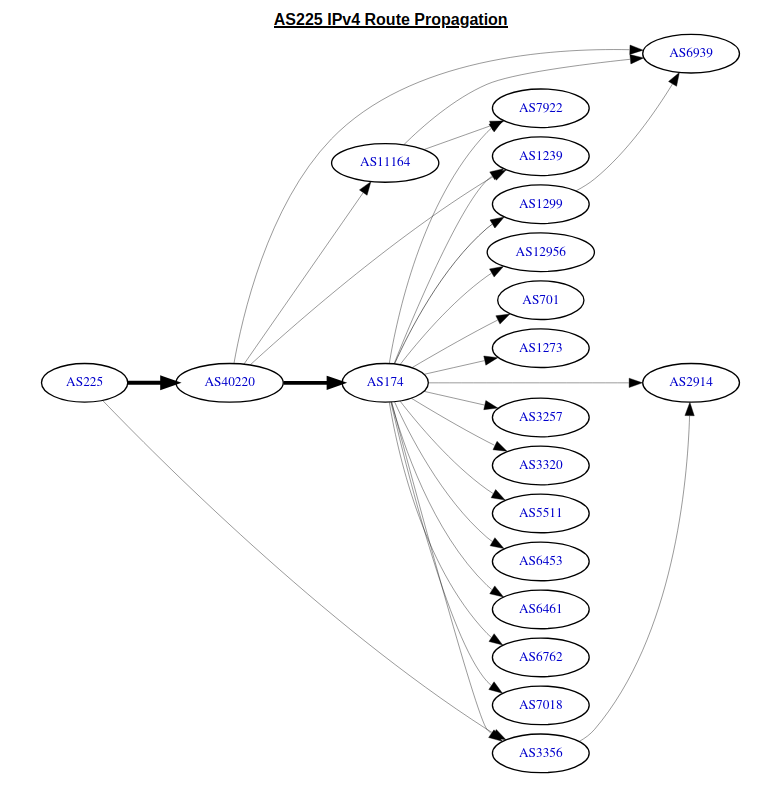
\includegraphics[width=0.5\textwidth]{../routing/as225-graph}
\end{frame}

\begin{frame}{AS40220}
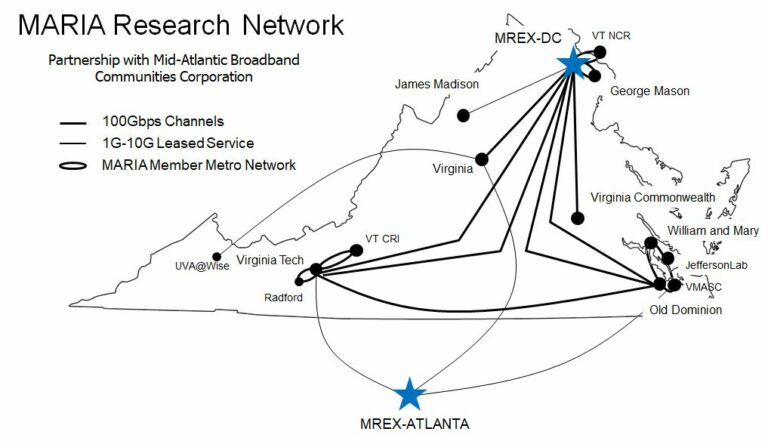
\includegraphics[height=0.8\textheight]{../routing/MARIA-Network-BW-768x441.jpg}
\end{frame}

\begin{frame}{}
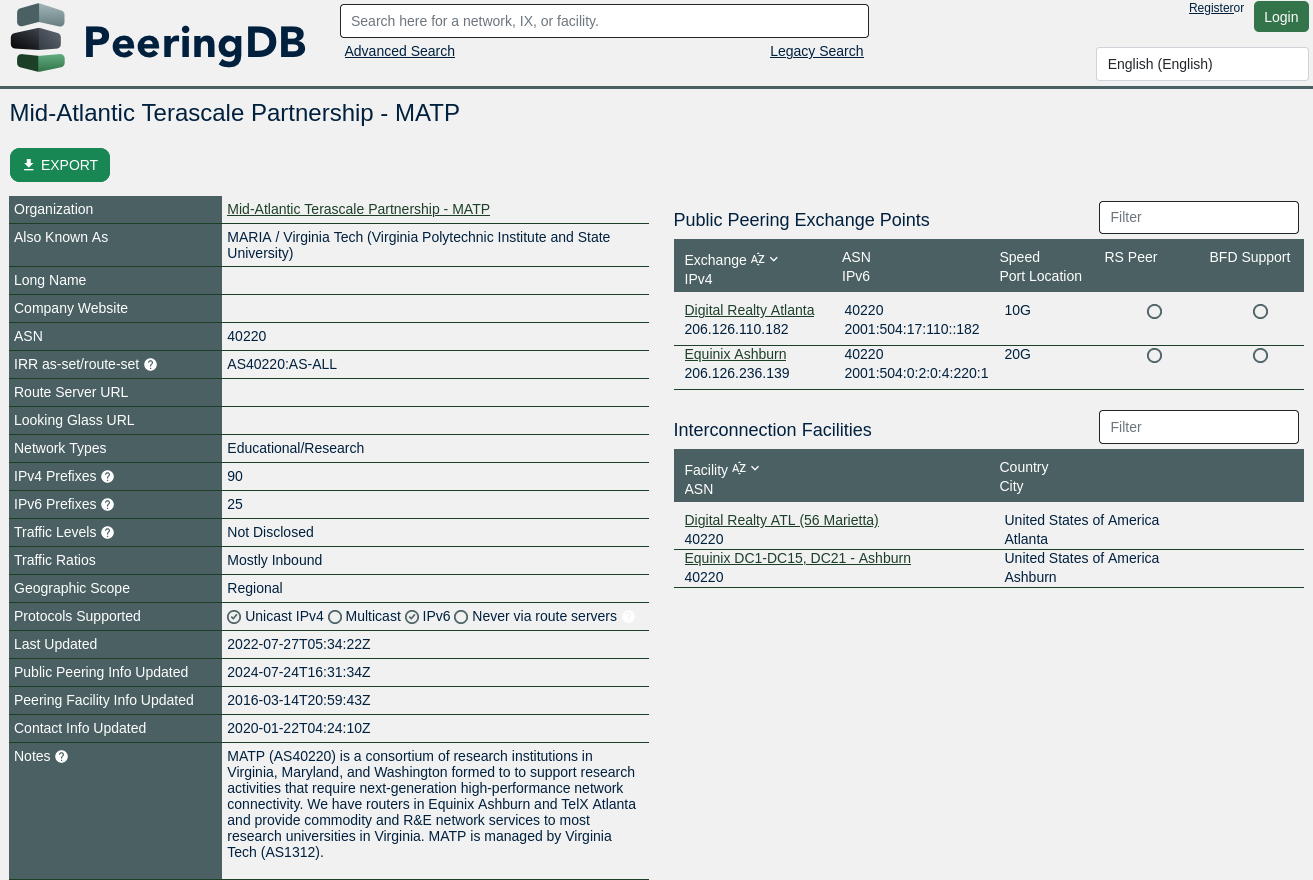
\includegraphics[width=0.95\textwidth]{../routing/as40220-peeringdb}
\end{frame}

\begin{frame}{AS3356}

\includegraphics[height=0.8\textheight]{../routing/lumen-webpage.png}
\end{frame}

\begin{frame}{AS3356 is a backup (8x AS prepending)}
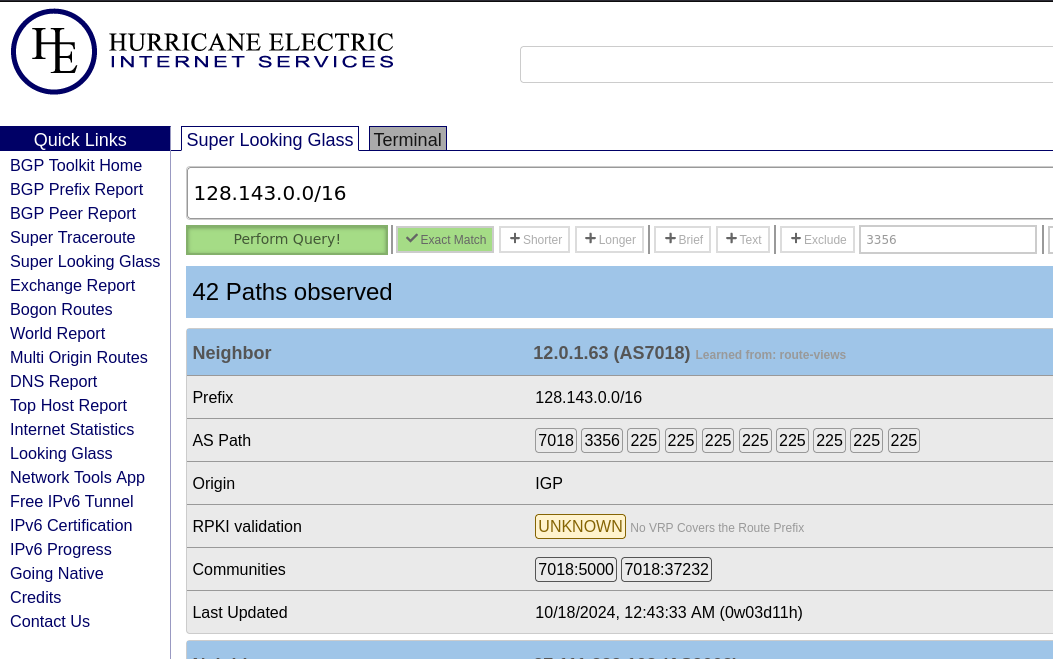
\includegraphics[height=0.8\textheight]{../routing/as3356-he-superlg.png}
\end{frame}


\subsection{internet exchanges, peeringdb}


\begin{frame}{peeringdb}
    \begin{itemize}
    \item \url{https://peeringdb.com} --- commonly used database of ASes and how to peer with them
    \item there is also -- ``whois'' records (from RIRs) for ASes, IP blocks with contact info
    \end{itemize}
\end{frame}

\begin{frame}{internet exchanges and route servers}
    \begin{itemize}
    \item internet exchange
        \begin{itemize}
        \item local network (typically within metro area) for connecting networks
        \item often run at and/or by `carrier-neutral' datacenter
        \item typically high bandwidth (10-100Gbps ports to network)
        \item provides connections when
        \end{itemize}
    \vspace{.5cm}
    \item route servers
        \begin{itemize}
        \item BGP servers run by internet exchange
        \item consolidates routes from participants
        \item goal: only need O($n$) BGP connections, not O($n^2$)
        \end{itemize}
    \end{itemize}
\end{frame}


\subsection{BGP communities}
\begin{frame}{BGP communities}
    \begin{itemize}
    \item routes sent via BGP can have `communities'
    \item extra information tagged on routes sent via BGP
    \vspace{.5cm}
    \item large ISPs have lists of communities their customers/peers can use
    \item \ldots and these affect how those routes are used
    \end{itemize}
\end{frame}

\begin{frame}{aside: Internet2}
    \begin{itemize}
    \item non-profit networking consortium
    \item operations major US University-focused network
    \item basically one of UVa's ISPs
    \end{itemize}
\end{frame}

\begin{frame}[fragile]{selected Internet2 BGP communities}
\begin{tikzpicture}
\node (a) {
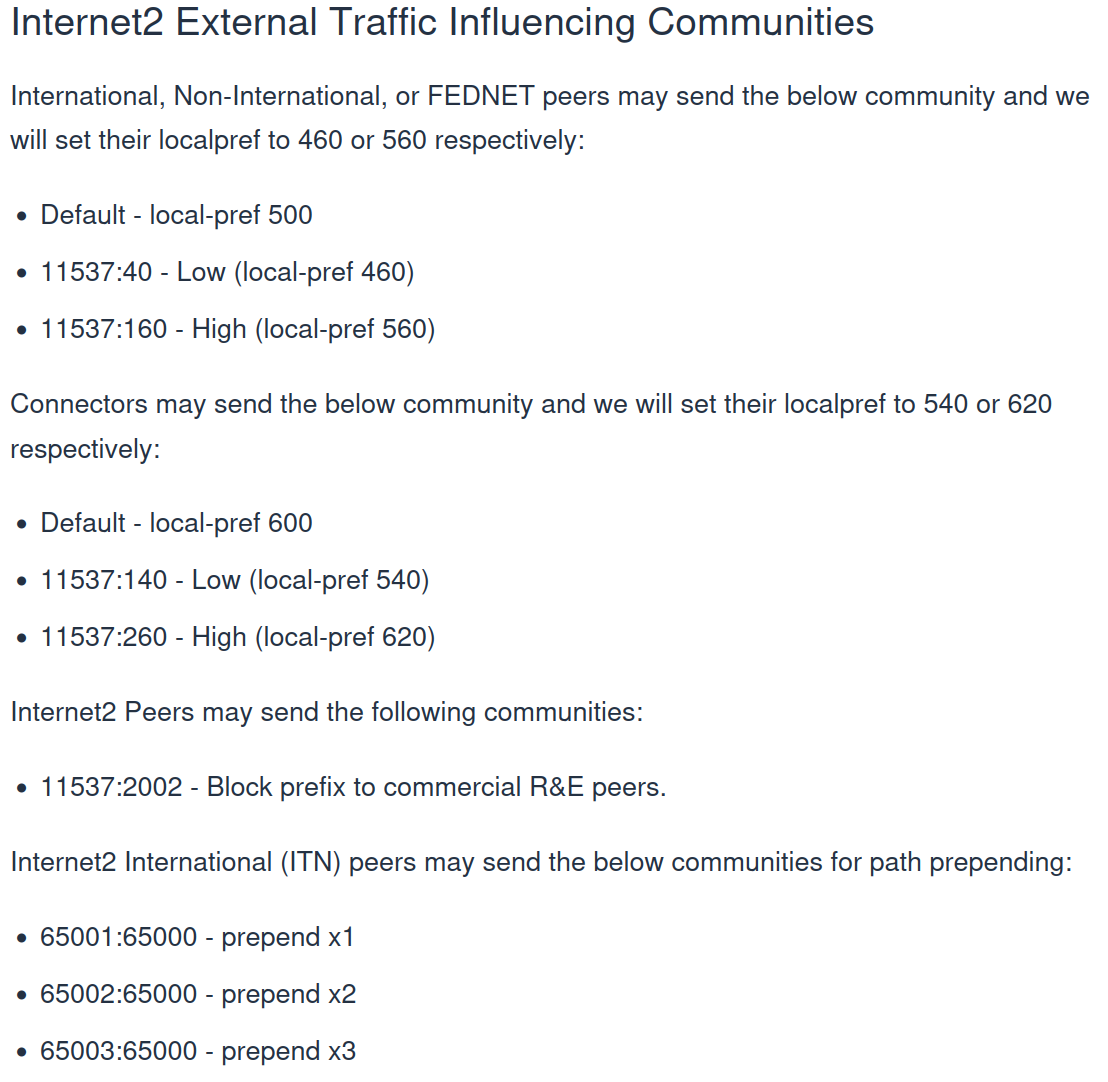
\includegraphics[width=0.49\textwidth]{../routing/i2-bgp-ext-comm}
};
\node[anchor=north west] (b) at (a.north east) {
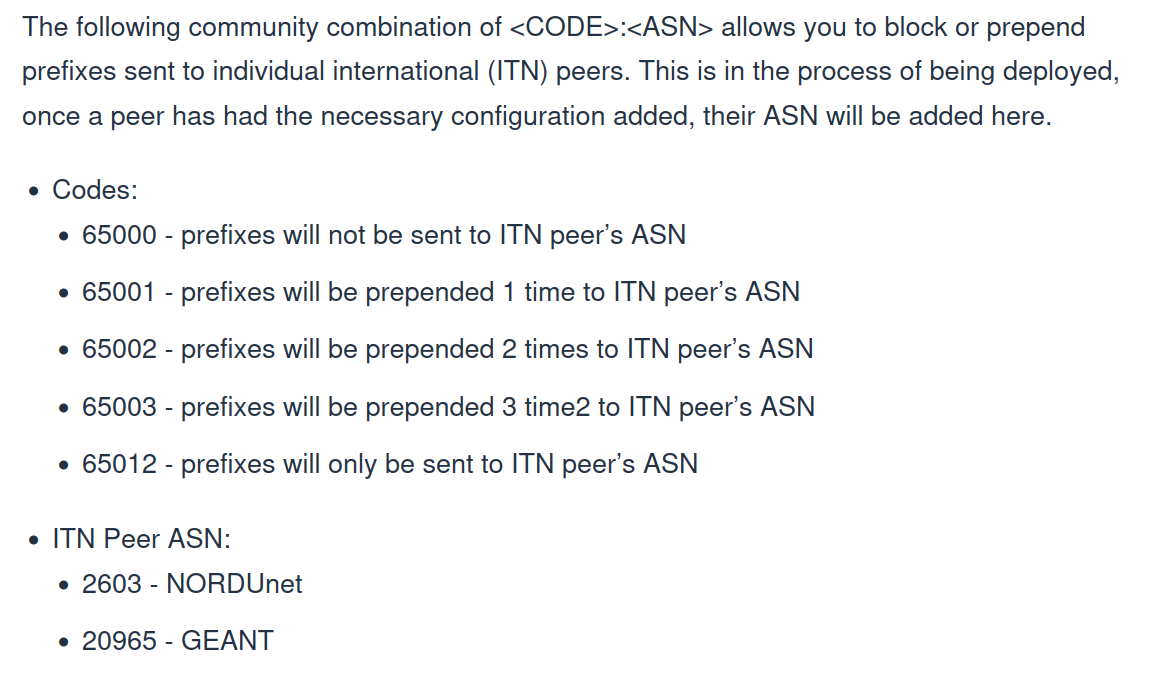
\includegraphics[width=0.39\textwidth]{../routing/i2-bgp-ext-comm2}
};
\node[anchor=north west] (c) at (b.south west) {
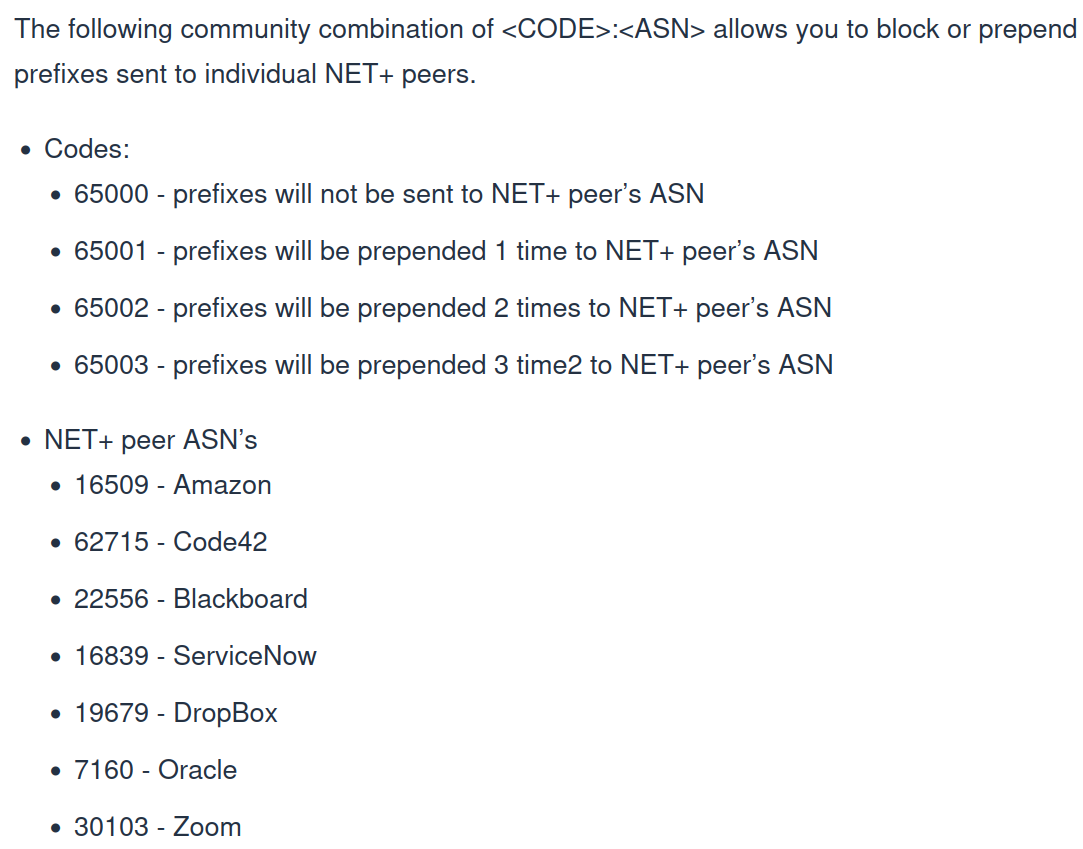
\includegraphics[width=0.39\textwidth]{../routing/i2-bgp-ext-comm3}
};
\end{tikzpicture}
{\fontsize{9}{10}\selectfont\url{https://noc.net.internet2.edu/knowledge/policy-statements/internet2-bgp-communities.html}}
\end{frame}

\begin{frame}{community options from prev slide}
\begin{itemize}
\item setting local-pref:
    \begin{itemize}
    \item you can decide how preferred your route is by Internet2
    \item maybe to make one primary, another secondary?
    \end{itemize}
\item blocking route from being sent to specific place
\item prepending Internet2's AS before forwarding prefix
    \begin{itemize}
    \item hopefully make that route less preferred by others
    \end{itemize}
\item prepending Internet2's AS before forwarding prefix to specific place
    \begin{itemize}
    \item hopefully make that route less preferred by that place
    \end{itemize}
\end{itemize}
\end{frame}

\begin{frame}{other things with communities}
    \begin{itemize}
    \item Internet2 also uses communities to mark\ldots
    \item what location routes were learned from
    \item what type of organization routes were learned from
    \item whether Internet2 is only allowed to use the route non-commerically or not
    \item \ldots
    \end{itemize}
\end{frame}



\subsection{BGP hijacking/fat fingers}

\begin{frame}{AS7007}
{\fontsize{8}{9}\selectfont\url{https://seclists.org/nanog/1997/Apr/444}}

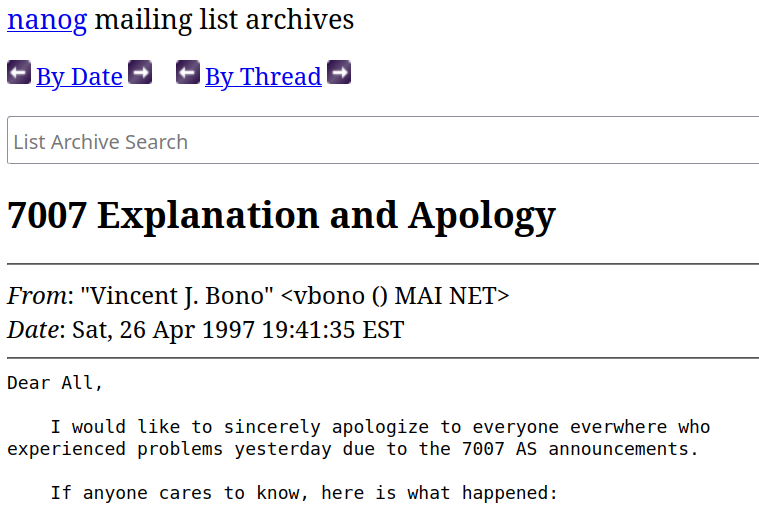
\includegraphics[width=0.4\textwidth]{../routing/as7007-1.png}
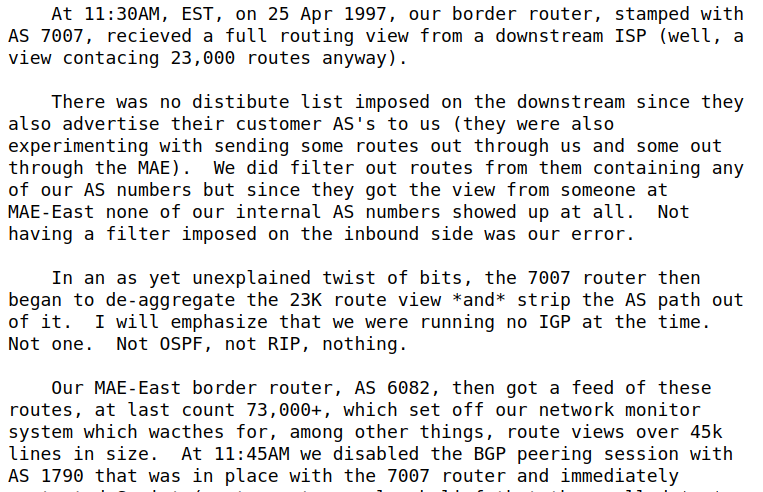
\includegraphics[height=0.4\textwidth]{../routing/as7007-2.png}
\end{frame}

\begin{frame}{2008 Pakistan Youtube}
\begin{itemize}
\item Pakistan Telecom recieved gov't order to block youtube
\item implemented by inserting route for YouTube's IP in internal network
\vspace{.5cm}
\item misconfiguration meant route was advertised on BGP
\item was more specific than YouTube's route, so made YouTube unreachablej
\end{itemize}
\end{frame}

\begin{frame}{timeline from RIPE NCC}
\begin{itemize}
\item {\tiny \url{https://www.ripe.net/about-us/news/youtube-hijacking-a-ripe-ncc-ris-case-study/}}
\item Youtube is announcing 208.65.152.0/22
\item 18:47Z: Pakistan Telecom starts announcing 208.65.153.0/24
\item 20:07Z: Youtube starts announcing 208.65.152.0/24
\item 20:18Z: Youtube starts announcing 208.65.152.0/25 and 208.65.152.128/25
\item 20:51Z: Pakistan Telecom's ISP forwards their announcements with additional copy of Pakistan Telecom's AS number
\item 21:01Z: Pakistan Telecom's ISP withdraws routes initiated by Pakistan Telecom (but not Pakistan Telecom's customers)
\end{itemize}
\end{frame}

\begin{frame}{BGP Hijacking targeted cryptocurrency stuff}
    \begin{itemize}
    \item KLAYswap (Feb 2022), Celer Bridge (Sep 2022)
    \item attackers intentionally redirected traffic to malicious version of services
    \item \ldots and stole money
    \vspace{.5cm}
    \item both probably spoofed the final AS number in AS path
    \item sometimes involved adding attacked IP range to routing registry
    \end{itemize}
\end{frame}

\begin{frame}{nation-states?}

\includegraphics[width=\textwidth]{../routing/china-tele-ars-tech}
\end{frame}


\subsection{validating routes / sBGP}
\begin{frame}{route security}
    \begin{itemize}
    \item historically, no verification routes announced by ``owner'' of IP addresses
    \vspace{.5cm}
    \item probably some ISPs filter
    \item effort to deploy RPKI --- public-key based scheme to verify routes
        \begin{itemize}
        \item checks that routes originated at correct AS
        \item doesn't verify intermediate ASes will forward correctly
        \end{itemize}
    \end{itemize}
\end{frame}

\begin{frame}{}
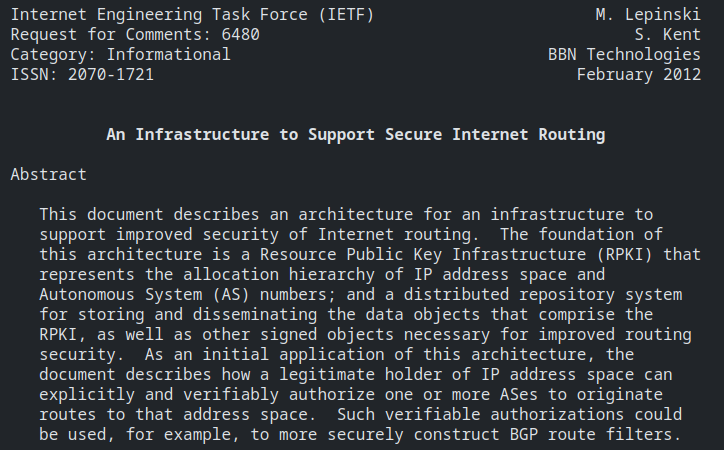
\includegraphics[height=\textheight]{../routing/rpki-rfc}
\end{frame}



\subsection{aside: partial tables}
\begin{frame}{partial tables}
    \begin{itemize}
    \item dealing with full Internet routing table is expensive
    \vspace{.5cm}
    \item common shortcut if you have a couple ISPs:
    \item keep `short' routes (example: short AS path)
    \item use default route for other cases
        \begin{itemize}
        \item to one of your ``primary'' ISPs
        \item maybe using ECMP
        \end{itemize}
    \end{itemize}
\end{frame}


\section{names versus addresses}
\usetikzlibrary{arrows.meta,calc,positioning,shapes.callouts,shapes.symbols}

\begin{frame}[label=nameAndAddr]{names and addresses}
\small
\begin{tabular}{l|l}
\textbf{name} & \textbf{address} \\\hline
\large\myemph{logical identifier} & \large\myemph{location/how to locate} \\
DNS name \texttt{www.virginia.edu} & IPv4 address \texttt{128.143.22.36} \\
DNS name \texttt{mail.google.com} & IPv4 address \texttt{216.58.217.69} \\
DNS name \texttt{mail.google.com} & IPv6 address \fontsize{10}{11}\selectfont\texttt{2607:f8b0:4004:80b::2005} \\
    DNS name \fontsize{9.5}{10.5}\selectfont\texttt{reiss-t3620.cs.virginia.edu} & IPv4 address \texttt{128.143.67.91} \\
~ & ~ \\
\end{tabular}
\end{frame}


\section{DNS hierarchy, caching}
\usetikzlibrary{arrows.meta,positioning,shapes.callouts}
\begin{frame}[fragile,label=dnsDD]{DNS: distributed database}
\begin{tikzpicture}
    \tikzset{
        >=Latex,
        comp box/.style={draw, thick, align=center, minimum width=1.5cm,minimum height=1.5cm},
        explain box/.style={draw=red,very thick, align=left},
        msg/.style={font=\small},
        cmd/.style={font=\small},
        my callout2/.style={draw,fill=blue!10!white,rectangle callout,callout absolute pointer=(#1),below right=5pt of {#1}}
    }
    \node[comp box] (my machine) at (0, 0) { my \\ machine };
    \node[comp box] (isp) at (6, 0) { ISP's \\ DNS server };
    \begin{visibleenv}<1>
        \node[my callout2=isp.south,fill=red!10,align=center,font=\small,anchor=north] at ([xshift=-2cm,yshift=-2cm]isp.south) {
            address sent to my machine \\
            when it connected to network
        };
    \end{visibleenv}
    \begin{visibleenv}<3->
    \node[comp box] (root) at (11, 2) { root \\ DNS server };
    \end{visibleenv}
    \begin{visibleenv}<4->
    \node[comp box] (edu) at (11, 0) { .edu \\ DNS server };
    \node[comp box] (virginia) at (11, -2) { virginia.edu \\ DNS server };
    \node[comp box] (cs) at (11, -4) { {\small cs.virginia.edu} \\ DNS server };
    \end{visibleenv}
    \begin{visibleenv}<2->
    \draw[very thick,<->] (my machine) -- (isp)
        coordinate[midway] (midpt);
    \node[my callout2=midpt,anchor=south,font=\fontsize{9}{10}\selectfont,align=left] at ([yshift=1cm]midpt) {
        address for \\ www.cs.virginia.edu?
    };
    \end{visibleenv}
    \begin{visibleenv}<5->
    \node[my callout2=midpt,anchor=north,font=\fontsize{9}{10}\selectfont,align=left] at ([yshift=-1cm]midpt) {
        www.cs.virginia.edu = \\
        128.143.67.11
    };
    \end{visibleenv}
    \foreach \n/\when in {root/3,edu/4,virginia/4,cs/4} {
        \draw[very thick,<->,alt=<\when->{}{invisible}] (isp) -- (\n.west) coordinate[midway] (midpt \n);
    }
    \begin{visibleenv}<3->
        \node[my callout2=midpt root,anchor=south,font=\fontsize{9}{10}\selectfont,align=left,
              alt=<5>{fill=red!10}] at ([yshift=1cm]midpt root) {
            www.cs.virginia.edu? \\
            try .edu server at \ldots
        };
        \begin{visibleenv}<5>
            \draw[very thick,dotted,red,<->] (isp) -- (root.west);
            \node[draw=red,very thick,fill=white,align=left,anchor=north,font=\small] at ([yshift=-3cm]midpt root) {
                .edu server doesn't change much \\
                optimization: \textit{cache} its address \\
                ~ \\
                check for updated version once in a while
            };
        \end{visibleenv}
    \end{visibleenv}
\end{tikzpicture}
\end{frame}


\usetikzlibrary{graphs,graphdrawing,fit}
\usegdlibrary{trees,layered}
\begin{frame}{DNS hierarchy}
\begin{tikzpicture}
\graph[
tree layout,
    level 1/.style={sibling distance=7cm},
    level 2/.style={sibling distance=3cm,nodes={font=\small}},
    level 3/.style={sibling distance=1cm,nodes={font=\small}},
] {
    root/"." -> { 
        com/"com" -> {comdot/"\ldots"},
        ,
        ,
        edu/"edu" -> {
            virginia/"virginia" -> {
                cs/"cs" -> {
                    kytos02,
                    www,
                    csdot/\ldots
                },
                ,
                ,
                engineering/"engineering",
                ,
                ,
                its/"its" -> {
                    canvas,
                    shibidp,
                    itsdot/\ldots
                },
            },
            ,
            ,
            vt/"vt",
            vcu/"vcu",
            edudot/"\ldots"
        },
        ,
        rootdot/"\ldots"
    };
};
\coordinate (place) at ([yshift=-4cm]root);
\begin{visibleenv}<1>
    \node[anchor=north,align=center] at (place) {
        hierarchy with single root
    };
\end{visibleenv}
\begin{visibleenv}<2>
    \foreach \x in {(root),(com),(edu),(vt),(vcu),
        (cs) (kytos02) (www) (csdot)} {
        \node[draw=red,very thick,inner sep=0mm,fit=\x] {};
    }
    \draw[red,very thick] (engineering.south west) |- (virginia.north east) |- (its.north) -| (itsdot.south east)
        -| cycle;
    \node[anchor=north,align=center] at (place) {
        divided into `zones' \\
        each with own set of authoritative servers
    };
\end{visibleenv}
\end{tikzpicture}
\end{frame}



\subsection{authoritative/recursive v not}
\begin{frame}{terms: authority, recursive}
    \begin{itemize}
    \item DNS server is \textit{authoritative} for X.Y.Z?
        \begin{itemize}
        \item (claims to be) official source of information for X.Y.Z
        \item not giving a cached version obtained from elsewhere
        \end{itemize}
    \item DNS server is a \textit{recursive resolver}?
        \begin{itemize}
        \item will contact other DNS servers to get answer
        \end{itemize}
    \vspace{.5cm}
    \item choice of whoever configures DNS server
    \end{itemize}
\end{frame}


\section{example}

\begin{frame}[fragile]{querying the root}
\begin{Verbatim}[fontsize=\scriptsize]
$ dig +trace +all www.cs.virginia.edu
...
edu.			172800	IN	NS	b.edu-servers.net.
edu.			172800	IN	NS	f.edu-servers.net.
edu.			172800	IN	NS	i.edu-servers.net.
edu.			172800	IN	NS	a.edu-servers.net.
...
b.edu-servers.net.	172800	IN	A	191.33.14.30
b.edu-servers.net.	172800	IN	AAAA	2001:503:231d::2:30
f.edu-servers.net.	172800	IN	A	192.35.51.30
f.edu-servers.net.	172800	IN	AAAA	2001:503:d414::30
...
;; Received 843 bytes from 198.97.190.53#53(h.root-servers.net) in 8 ms
...
\end{Verbatim}
\end{frame}

\begin{frame}[fragile]{querying the edu}
\begin{Verbatim}[fontsize=\scriptsize]
$ dig +trace +all www.cs.virginia.edu
...
virginia.edu.		172800	IN	NS	nom.virginia.edu.
virginia.edu.		172800	IN	NS	uvaarpa.virginia.edu.
virginia.edu.		172800	IN	NS	eip-01-aws.net.virginia.edu.
nom.virginia.edu.	172800	IN	A	128.143.107.101
uvaarpa.virginia.edu.	172800	IN	A	128.143.107.117
eip-01-aws.net.virginia.edu. 172800 IN	A	44.234.207.10
;; Received 165 bytes from 192.26.92.30#53(c.edu-servers.net) in 40 ms
...
\end{Verbatim}
\end{frame}
\begin{frame}[fragile]{querying virginia.edu+cs.virginia.edu}
\begin{Verbatim}[fontsize=\scriptsize]
$ dig +trace +all www.cs.virginia.edu
...
cs.virginia.edu.	3600	IN	NS	coresrv01.cs.virginia.edu.
coresrv01.cs.virginia.edu. 3600	IN	A	128.143.67.11
;; Received 116 bytes from 44.234.207.10#53(eip-01-aws.net.virginia.edu) in 72 ms

www.cs.Virginia.EDU.	172800	IN	A	128.143.67.11
cs.Virginia.EDU.	172800	IN	NS	coresrv01.cs.Virginia.EDU.
coresrv01.cs.Virginia.EDU. 172800 IN	A	128.143.67.11
;; Received 151 bytes from 128.143.67.11#53(coresrv01.cs.virginia.edu) in 4 ms
\end{Verbatim}
\end{frame}

\begin{frame}[fragile]{querying typical ISP's resolver}
\begin{Verbatim}[fontsize=\scriptsize]
$ dig www.cs.virginia.edu
...
;; ANSWER SECTION:
www.cs.Virginia.EDU.	  7183	IN	A	128.143.67.11
..
\end{Verbatim}
\end{frame}


\subsection{aside: presentation format}
\begin{frame}{DNS presentation format}
    \begin{itemize}
    \item DNS uses compact binary format we'll talk about later
    \vspace{.5cm}
    \item also has standardized `presentation format' that \texttt{dig} uses (roughly)
    \item format is used for DNS server configuration files
    \end{itemize}
\end{frame}


\subsection{TTLs and changing things}
\begin{frame}{DNS time-to-live}
    \begin{itemize}
    \item need some way to remove out-of-date DNS records
    \vspace{.5cm}
    \item DNS solution: time-to-live
    \item number of seconds record is valid for
    \end{itemize}
\end{frame}


\begin{frame}{DNS exercise (1)}
    \begin{itemize}
    \item ``www.cs.virginia.edu is 128.148.67.11 \myemph{for next 86400 seconds}''
    \item (given record above)
    if sysadmin changes IP address DNS server returns for www.cs.virginia.edu,
    then what will happen to machines accessing website?
        \begin{itemize}
        \item A. they'll start using the new address after 86400 seconds, and use the old one before then.
        \item B. different machines will use the new address at different times, but no longer than 86400 seconds from when it changes
        \item C. machines will start using the new address almost immediately, but after some small delay after it is changed
        \item D. machines may keep using the old address until they are rebooted
        \item E. something else?
        \end{itemize}
    \end{itemize}
\end{frame}

\begin{frame}{DNS exercise (2)}
    \begin{itemize}
    \item if sysadmin wants to change the IP address of www.cs.virginia.edu,
            how do they do this without downtime?
    \vspace{.5cm}
    \item they can change the IP address the server returns and/or the time-to-live?
    \item what should they change and when to smoothly transition to a new address?
    \end{itemize}
\end{frame}

\begin{frame}{DNS exercise (3)}
    \begin{itemize}
    \item suppose initially
        \begin{itemize}
        \item *.foo.com DNS server (`nameserver') = 10.2.3.4, valid 200 s
        \item www.foo.com = 10.1.2.3, valid 100 s
        \end{itemize}
    \item if at time 0 seconds, changed to:
        \begin{itemize}
        \item *.foo.com DNS server = 10.3.4.5, valid 100 s
        \item www.foo.com DNS server = 10.3.5.1, valid 400 s
        \end{itemize}
    \item ex 0: when will new DNS server/www.foo.com start being used?
    \item ex 1: when can we shut down old DNS server?
    \item ex 2: when can we shut down old www.foo.com?
    \end{itemize}
\end{frame}


\section{root servers}
\begin{frame}{root servers (1)}
(from IANA's website)
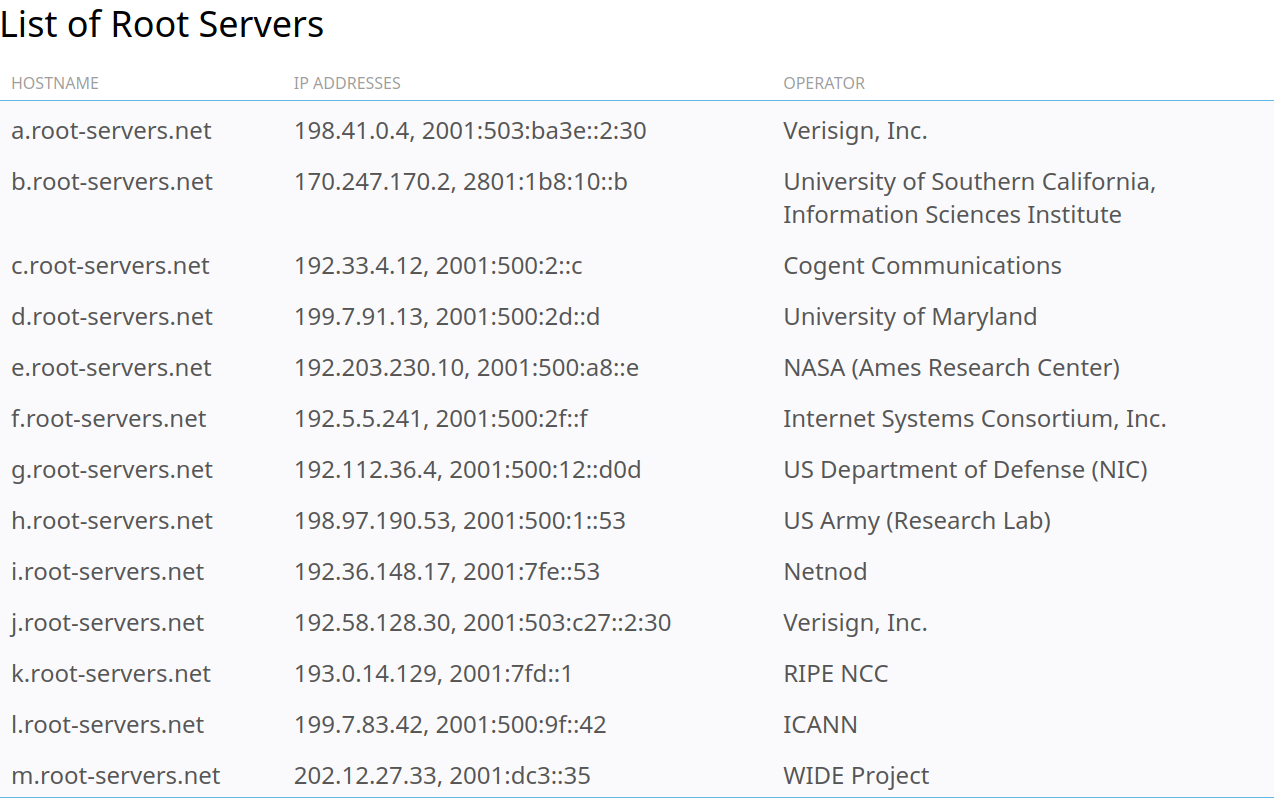
\includegraphics[height=0.8\textheight]{../dns/iana-root-server-list}
\end{frame}

\begin{frame}{root servers (2)}
(from root-servers.org)
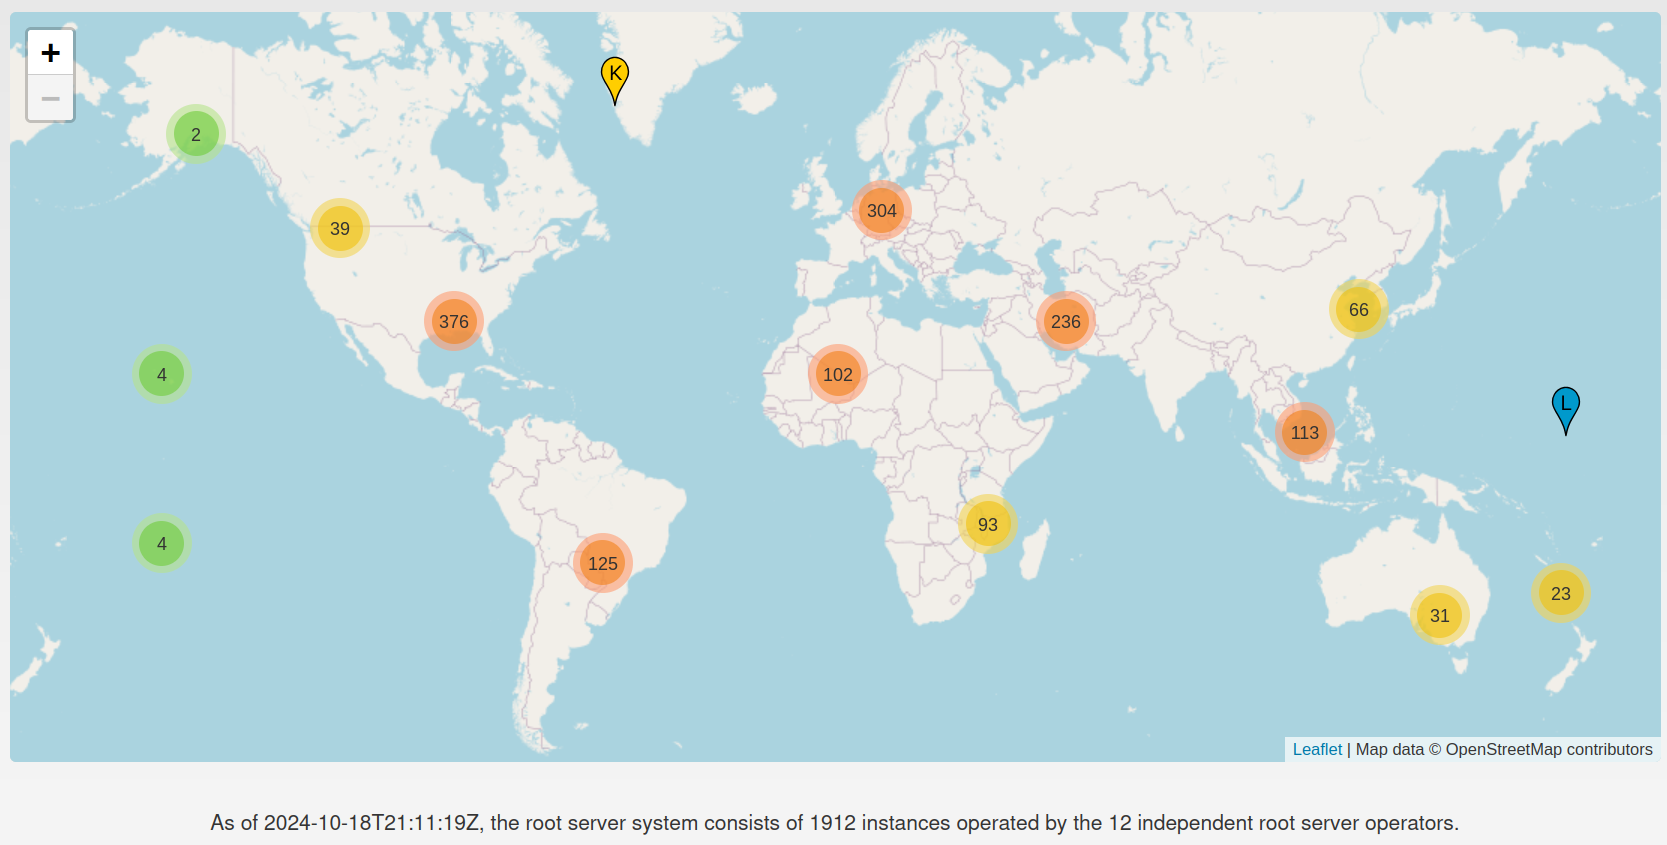
\includegraphics[width=0.9\textwidth]{../dns/root-servers-map}
\end{frame}

\begin{frame}{anycast root servers}
    \begin{itemize}
    \item many root servers have multiple separate sites
    \item \ldots but one IPv4/IPv6 address
    \vspace{.5cm}
    \item which one you get = which one routed to
    \item multiple sites with BGP announcements for IP
        \begin{itemize}
        \item often with care taken to limit how far route goes
        \end{itemize}
    \item idea called `anycast'
        \begin{itemize}
        \item get to `any' of several servers
        \end{itemize}
    \item also used for some public recursive DNS servers
        \begin{itemize}
        \item 1.1.1.1 (CloudFlare), 8.8.8.8 (Google), 208.67.222.222 (Cisco), \ldots
        \end{itemize}
    \end{itemize}
\end{frame}


\section{registrars versus registries}
\begin{frame}{DNS registries}
    \begin{itemize}
    \item IANA and affiliates publish root zone file
        \begin{itemize}
        \item same organization as for IP address, AS numbers
        \item (but domain names are lot more politically active)
        \end{itemize}
    \item For usable top-level domains, there are \textit{registries}:
        \begin{itemize}
        \item VeriSign (VA company) for \texttt{COM}, \texttt{NET}
        \item Educause (non-profit) for \texttt{EDU}
        \item Registry Services, LLC (under contract with the US Dept of Commerce) for \texttt{US}
        \item \ldots
        \end{itemize}
    \item many registries allow for many \textit{registrars} who can sell new domains
    \end{itemize}
\end{frame}


\section{DNS record format}
\usetikzlibrary{decorations.pathreplacing,decorations.pathmorphing,arrows.meta}

\begin{frame}{DNS resource records}
\begin{itemize}
\item resource record (RR) = single DNS database `entry'
\item has standard text and binary representation
    \begin{itemize}
    \item text used for server config files and display
    \item binary representation used for network protocol
    \end{itemize}
\end{itemize}
\end{frame}

\begin{frame}{DNS record example (text)}
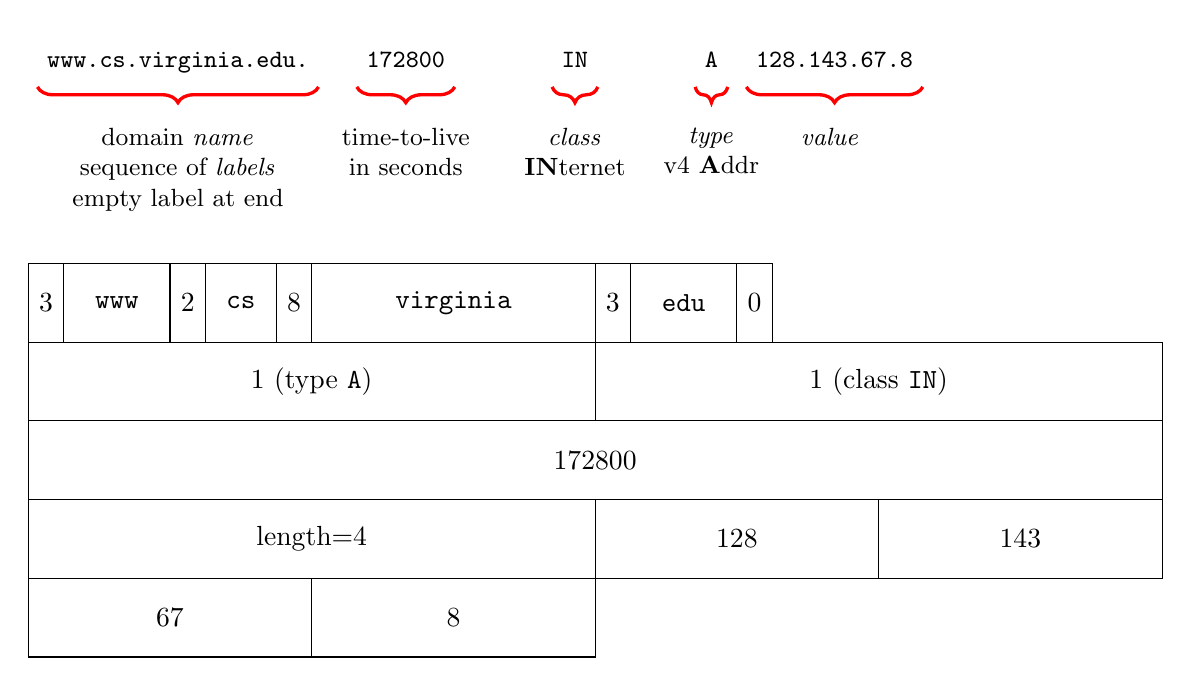
\begin{tikzpicture}
\matrix[ampersand replacement=\&,every node/.style={font=\small\tt\strut},column sep=0.5cm,anchor=north west] at (0,0) {
    \node (www) {www.cs.virginia.edu.}; \& \node (www ttl) {172800}; \&[.75cm]
    \node (www in) {IN}; \&[.75cm] \node (www a) {A}; \&[-.25cm]
    \node (www value) {128.143.67.8}; \\
};
\tikzset{
    mymark/.style={decorate,decoration={brace,amplitude=2mm},draw=red,very thick},
    mymark label/.style={draw=none,align=center,inner sep=5mm,font=\small},
}
\draw[mymark] (www.south east) -- (www.south west)
    node[below,midway,mymark label] {
        domain \textit{name} \\
        sequence of \textit{labels} \\
        empty label at end 
    };
\draw[mymark] (www ttl.south east) -- (www ttl.south west)
    node[below,midway,mymark label] {
        time-to-live \\
        in seconds
    };

\draw[mymark] (www in.south east) -- (www in.south west)
    node[below,midway,mymark label] {
        \textit{class} \\
        \textbf{IN}ternet
    };
\draw[mymark] (www a.south east) -- (www a.south west)
    node[below,midway,mymark label] {
        \textit{type} \\
        v4 \textbf{A}ddr
    };
\draw[mymark] (www value.south east) -- (www value.south west)
    node[below,midway,mymark label] {
        \textit{value}
    };
\begin{scope}[yshift=-3cm,x=0.45cm]
    \draw (0, 0) rectangle ++(1, -1) node[midway] {3};
    \draw (1, 0) rectangle ++(3, -1) node[midway] {\texttt{www}};
    \draw (4, 0) rectangle ++(1, -1) node[midway] {2};
    \draw (5, 0) rectangle ++(2, -1) node[midway] {\texttt{cs}};
    \draw (7, 0) rectangle ++(1, -1) node[midway] {8};
    \draw (8, 0) rectangle ++(8, -1) node[midway] {\texttt{virginia}};
    \draw (16, 0) rectangle ++(1, -1) node[midway] {3};
    \draw (17, 0) rectangle ++(3, -1) node[midway] {\texttt{edu}};
    \draw (20, 0) rectangle ++(1, -1) node[midway] {0};
    \draw (0, -1) rectangle ++(16, -1) node[midway] { 1 (type \texttt{A}) };
    \draw (16, -1) rectangle ++(16, -1) node[midway] { 1 (class \texttt{IN}) };
    \draw (0, -2) rectangle ++(32, -1) node[midway] {172800 };
    \draw (0, -3) rectangle ++(16, -1) node[midway] { length=4 };
    \draw (16, -3) rectangle ++(8, -1) node[midway] { 128 };
    \draw (24, -3) rectangle ++(8, -1) node[midway] { 143 };
    \draw (0, -4) rectangle ++(8, -1) node[midway] { 67 };
    \draw (8, -4) rectangle ++(8, -1) node[midway] { 8 };
\end{scope}
\end{tikzpicture}
\end{frame}

\begin{frame}{DNS name format}
\begin{tikzpicture}
\begin{scope}[x=0.45cm]
    \draw (0, 0) rectangle ++(1, -1) node[midway] {3};
    \draw (1, 0) rectangle ++(3, -1) node[midway] {\texttt{www}};
    \coordinate (ptr end) at (4.5, -1);
    \draw (4, 0) rectangle ++(1, -1) node[midway] {2};
    \draw (5, 0) rectangle ++(2, -1) node[midway] {\texttt{cs}};
    \draw (7, 0) rectangle ++(1, -1) node[midway] {8};
    \draw (8, 0) rectangle ++(8, -1) node[midway] {\texttt{virginia}};
    \draw (16, 0) rectangle ++(1, -1) node[midway] {3};
    \draw (17, 0) rectangle ++(3, -1) node[midway] {\texttt{edu}};
    \draw (20, 0) rectangle ++(1, -1) node[midway] {0};
    \node[anchor=north] at (16, -1) {\ldots};
\end{scope}
\begin{scope}[x=0.45cm,yshift=-1.5cm,xshift=1.5cm]
    \draw (0, 0) rectangle ++(1, -1) node[midway,font=\small\tt] {10};
    \draw (1, 0) rectangle ++(10, -1) node[midway] {\texttt{coresrv01a}};
    \draw (11, 0) rectangle ++(2, -1);
    \draw[fill=black!30] (11, 0) rectangle ++ (0.25, -1);
    \coordinate (ptr base) at (12, -.5);
\end{scope}
\draw[very thick,-Latex] (ptr base) |- ([yshift=-.4cm]ptr end) -- (ptr end);
\end{tikzpicture}
\begin{itemize}
\item zero or more: length of $K>0$ followed by $K$ character case-insensitive \textit{label}
    \begin{itemize}
    \item labels limited to 64 bytes
    \end{itemize}
\item then either:
    \begin{itemize}
    \item length of $0$ to indicate end-of-name \textit{or}
    \item ``pointer'' to earlier name in message
        \begin{itemize}
        \item pointer encoded as \texttt{0xc000} + byte number in message (big endian)
        \item upper two bits being set prevents confusion with length
        \end{itemize}
    \end{itemize}
\end{itemize}
\end{frame}



\section{common record types}
\begin{frame}{selected RR types}
\begin{tabular}{l|l|l|p{6cm}}
text & id & purpose & data format \\ \hline
\texttt{A} & 1 & IPv4 address & 32-bit integer (big-endian) \\
\texttt{AAAA} & 28 & IPv6 address & 128-bit integer (big-endian) \\
\texttt{NS} & 2 & authoritative name server & domain name \\
\texttt{CNAME} & 5 & `canonical name' & domain name \\
\texttt{TXT} & 16 & text string & arbitrary string \\
\texttt{SRV} & 33 & service location & priority, weight, domain name, port \\
\end{tabular}
\end{frame}

\begin{frame}[fragile]{CNAME}
\begin{itemize}
\item CNAME = delegate name to another name
\end{itemize}
\begin{Verbatim}[fontsize=\small]
canvas.its.virginia.edu. 2711   IN      CNAME   \
    universityofvirginia-vanity.instructure.com.
universityofvirginia-vanity.instructure.com. 238 IN CNAME \
    canvas-pdx-prod-c354-1908777142.us-west-2.elb.amazonaws.com.
canvas-pdx-prod-c354-1908777142.us-west-2.elb.amazonaws.com. 2 IN A 34.208.211.157
canvas-pdx-prod-c354-1908777142.us-west-2.elb.amazonaws.com. 2 IN A 44.238.73.244
canvas-pdx-prod-c354-1908777142.us-west-2.elb.amazonaws.com. 2 IN A 52.26.9.245
\end{Verbatim}
\begin{itemize}
\item connecting to canvas.its.virginia.edu?
\item use one of 34.208.211.157, 44.238.73.244, 52.26.9.245
\end{itemize}
\end{frame}

\begin{frame}[fragile]{NS}
\begin{Verbatim}[fontsize=\small]
virginia.edu. 3600    IN      NS      uvaarpa.virginia.edu.
virginia.edu. 3600    IN      NS      nom.virginia.edu.
virginia.edu. 3600    IN      NS      eip-01-aws.net.virginia.edu.
\end{Verbatim}
\begin{itemize}
\item these three servers are authoritative for virginia.edu
\item (but need their A or AAAA records to actually contact them)
\end{itemize}
\end{frame}

\begin{frame}[fragile]{SRV}
\begin{Verbatim}
_ldap._tcp.virginia.edu. 600    IN      SRV     0 100 389 vadcv4.virginia.edu.
_ldap._tcp.virginia.edu. 600    IN      SRV     0 100 389 vadc5.virginia.edu.
\end{Verbatim}
\begin{itemize}
\item virginia.edu's LDAP servers are vadcv4.virginia.edu port 389 and vadc5.virginia.edu port 389
\item (LDAP = Lightweight Directory Access Protocol)
    \begin{itemize}
    \item example: lookup email ID by name
    \end{itemize}
\end{itemize}
\end{frame}

\begin{frame}{SRV records were late\ldots}
\begin{itemize}
\item SRV records seem like something we'd use all the time\ldots
\item but only used with a few protocols
\item why?
\vspace{.5cm}
\item SRV records added late (1996--2000)
\item sending email already had its own record type (MX)
\item poor support for querying them in standard networking libraries
\item hard to get access to add them in many organizations
\end{itemize}
\end{frame}

\begin{frame}[fragile]{dig virginia.edu txt}
\begin{Verbatim}[fontsize=\fontsize{8}{9}]
virginia.edu.           3548    IN      TXT     "google-site-verification=zEwuk4FIG8_vtv2BZJOD6IWzg9JbNiJPH9mQdPNCXRw"
virginia.edu.           3548    IN      TXT     "cisco-ci-domain-verification=268b991de3589451b38fcfeaa99473f8e4fb2522f96a1b478e04ec1bd5a25ff9"
virginia.edu.           3548    IN      TXT     "miro-verification=9f3238c881466b3ccb99c4347b99e5504eafc118"
virginia.edu.           3548    IN      TXT     "MS=ms40126609"
virginia.edu.           3548    IN      TXT     "onetrust-domain-verification=d901adf09116474c89790a9752e0046c"
virginia.edu.           3548    IN      TXT     "google-site-verification=rePHmrM7FEfSw62DHq9TpuMFUw66J6hgpFFh5cq89IM"
virginia.edu.           3548    IN      TXT     "v=spf1 a mx ip4:52.254.56.82 ip4:52.137.91.139 ip4:128.143.125.90 ip4:128.143.125.91 include:spf.protection.outlook.com include:_spf.google.com include:spf.elluciancloud.com ~all"
virginia.edu.           3548    IN      TXT     "docusign=6547d080-1c40-427c-8736-fafa466ff73f"
virginia.edu.           3548    IN      TXT     "apple-domain-verification=zllSamqSFAw4lNQo"
virginia.edu.           3548    IN      TXT     "v=msv1 t=537499f256ea46bd386f7543d18d28"
virginia.edu.           3548    IN      TXT     "atlassian-domain-verification=zeQ45p2Vl1fXekKYCzmq4ONEpDEkGKx3Y8Qzqe/8YV2ibzq6DLImIdTNw9Cv4lda"
virginia.edu.           3548    IN      TXT     "00256316"
virginia.edu.           3548    IN      TXT     "yYMwnn+VY4w6aVf+cE4888ppz+MDXBKnaI0m5eteiMGgwWIBTOgA6aTSJM4QYRG6s49MnR2Fj0grzaOKokmCow=="
virginia.edu.           3548    IN      TXT     "apple-domain-verification=mROwKUEMfwLBfltC"
virginia.edu.           3548    IN      TXT     "e2ma-verification=rx8eb"
virginia.edu.           3548    IN      TXT     "ZOOM_verify_PuU-eQzyQ7ONrij_vTP72A"
virginia.edu.           3548    IN      TXT     "sending_domain1023271=f4a69653389ff4543a64e982f1cbc2e9db30eab95cccfb8be58d883ce7849448"
\end{Verbatim}
\end{frame}

\begin{frame}{TXT record usage}
\begin{itemize}
\item TXT records `just' hold arbitrary strings
\item lots of machine-based usage of TXT records
\item probably in part because it's too slow/hard to add new record types
\end{itemize}
\end{frame}

\begin{frame}[fragile]{TXT example: SPF}
\begin{Verbatim}[fontsize=\small]
virginia.edu. 3548    IN      TXT "v=spf1 a mx
    ip4:52.254.56.82 ip4:52.137.91.139
    ip4:128.143.125.90 ip4:128.143.125.91
    include:spf.protection.outlook.com
    include:_spf.google.com
    include:spf.elluciancloud.com ~all"
\end{Verbatim}
\begin{itemize}
\item SPF protocol for specifying who can send email from domain
\item why in TXT record instead of its own type?
\end{itemize}
\end{frame}

\begin{frame}{RFC 6686, Appendix A excerpt} 
\fontsize{13}{14}\selectfont
At the time of SPF's initial development, the prospect of getting an
RRTYPE allocated for SPF was not seriously considered, partly because
doing so had high barriers to entry\ldots.

\vspace{.5cm}

Later, after RRTYPE 99 was assigned \ldots
a plan was put into place to effect a gradual
transition to using RRTYPE 99 instead of using RRTYPE 16.
This plan failed to take effect for four primary reasons:\ldots

\vspace{.5cm}

1.\ldots existing nameservers (and, in fact, DNS-aware firewalls) would drop or
reject requests for unknown RRTYPEs \ldots

\vspace{.5cm}

2. many DNS provisioning tools \ldots
   were, and still are, typically lethargic about
   adding support for new RRTYPEs

\vspace{.5cm}

\ldots
\end{frame}


\section{primary, secondary, zone xfers}
\begin{frame}{primary and secondary servers}
\begin{itemize}
\item usually have multiple DNS servers for each zone
    \begin{itemize}
    \item needed to handle outages
    \end{itemize}
\item DNS protocol supports \textit{zone transfers} to synchronize them
    \begin{itemize}
    \item DNS query for type \texttt{AXFR} returns all RRs as special case
    \item (most public DNS servers block this from `normal'users)
    \end{itemize}
\item one server designed as `primary'; others are `secondary'
\item special SOA (start of authority) record provides metadata about zone
    \begin{itemize}
    \item name of primary server to contact
    \item serial number for current version (to quickly check if update)
    \item how long to wait between updates, etc.
    \end{itemize}
\end{itemize}
\end{frame}
 % FIXME: more detail?

\section{DNS query+answer format}
\begin{frame}{DNS messages (1)}
    \begin{itemize}
    \item client sends query to server
    \item server responds with response
    \vspace{.5cm}
    \item response and query have same format
        \begin{itemize}
        \item but different fields set/used
        \end{itemize}
    \end{itemize}
\end{frame}

\begin{frame}{DNS header}
\begin{tikzpicture}
\tikzset{
    blabel/.style={font=\small},
    blabel alt/.style={font=\fontsize{9}{10}\selectfont},
    flag/.style={alt=<2>{fill=red!10}},
    opcode/.style={alt=<3>{fill=red!10}},
    rcode/.style={alt=<4>{fill=red!10}},
}
\begin{scope}[yshift=0cm,x=0.45cm]
    \draw (0, 0) rectangle ++(16, -1) node[midway,blabel] {ID};
    \draw[flag] (16, 0) rectangle ++(1, -1) node[midway,blabel alt] {QR};
    \draw[opcode] (17, 0) rectangle ++(4, -1) node[midway,blabel] {opcode};
    \draw[flag] (21, 0) rectangle ++(1, -1) node[midway,blabel alt] {AA};
    \draw[flag] (22, 0) rectangle ++(1, -1) node[midway,blabel alt] {TC};
    \draw[flag] (23, 0) rectangle ++(1, -1) node[midway,blabel alt] {RD};
    \draw[flag] (24, 0) rectangle ++(1, -1) node[midway,blabel alt] {RA};
    \draw (25, 0) rectangle ++(1, -1) node[midway,blabel] {\tt 0};
    \draw[flag] (26, 0) rectangle ++(1, -1) node[midway,blabel alt] {AD};
    \draw[flag] (27, 0) rectangle ++(1, -1) node[midway,blabel alt] {CD};
    \draw[rcode] (28, 0) rectangle ++(4, -1) node[midway,blabel] {RCODE};
    \draw (0, -1) rectangle ++(16, -1) node[midway,blabel] {QDCOUNT (0 or 1)};
    \draw (16, -1) rectangle ++(16, -1) node[midway,blabel] {ANCOUNT};
    \draw (0, -2) rectangle ++(16, -1) node[midway,blabel] {NSCOUNT};
    \draw (16, -2) rectangle ++(16, -1) node[midway,blabel] {ARCOUNT};
    \draw (0, -3) rectangle ++(32, -1.5) node[midway,blabel] {QDCOUNT questions};
    \draw (0, -4.5) rectangle ++(32, -1.5) node[midway,blabel] {
            ANCOUNT+NSCOUNT+ARCOUNT RRs
    };
    \coordinate (mark low) at (16, -2.1);
\end{scope}
\tikzset{
    explain box low/.style={at={(mark low)},draw=red,very thick,align=left,anchor=north,fill=white},
    explain box low2/.style={at={([yshift=-2cm]mark low)},
        font=\small,draw=red,very thick,align=left,anchor=north,fill=white},
}
    \begin{visibleenv}<2>
    \node[explain box low2] {
        `flags' \\
        QR = 1 if query, 0 if response \\
        AA = 1 if authoritative \\
        TC = 1 if truncated (packet size limit) \\
        RD = 1 if query wants recursion (contact other servers) \\
        RA = 1 if server supports recursion  \\
        ~ \\
        DNSSEC (PKI for DNS) additions: \\
        AD = 1 if verified cryptographically (`authentic data') \\
        CD = 1 if no cryptographic check requested (`checking disabled') \\
    };
    \end{visibleenv}
    \begin{visibleenv}<3>
    \node[explain box low] {
        opcode \\
        0 for query \\
        some other operations
    };
    \end{visibleenv}
    \begin{visibleenv}<4>
    \node[explain box low] {
        response code, 0 for no error
    };
    \end{visibleenv}
\end{tikzpicture}
\end{frame}

\begin{frame}{caching `domain name does not exist'}
    \begin{itemize}
    \item when domain does not exist (RCODE=3, ``NXDOMAIN''):
    \vspace{.5cm}
    \item (RFC 2308)
    \item response should include SOA record
        \begin{itemize}
        \item recall: indicates primary server for zone and how often secondaries should update
        \end{itemize}
    \item can cache NXDOMAIN based on minimum of TTL and SOA record's update frequency
    \end{itemize}
\end{frame}

\begin{frame}{DNS message}
    \begin{itemize}
    \item header
    \item 0 or 1 question
        \begin{itemize}
        \item domain name + class + type
        \item (RR without TTL or value)
        \item special type values for ANY, some other things
        \end{itemize}
    \item ANCOUNT RRs in `answer section':
        \begin{itemize}
        \item CNAMEs (even if that's not the question type)
        \item matches for domain name (or CNAME) + class + type 
        \end{itemize}
    \item NSCOUNT+ARCOUNT RRs in `authority section' and `additional section
        \begin{itemize}
        \item not always included; usually NS or SOA records plus corresponding A/AAAA recods
        \end{itemize}
    \end{itemize}
\end{frame}


\section{DNS over UDP, TCP}
% size limitations
\begin{frame}{DNS over \ldots}
    \begin{itemize}
    \item UDP port 53
        \begin{itemize}
        \item send DNS message
        \item reply with DNS message back
        \end{itemize}
    \item TCP port 53
        \begin{itemize}
        \item send length (2B, big endian) + message
        \item reply with length (2B, big endian) + message
        \item (+ repeat)
        \end{itemize}
    \item over HTTPS (RFC 8484)
        \begin{itemize}
        \item using \url{https://server/dns-query}
        \end{itemize}
    \end{itemize}
\end{frame}

\begin{frame}[fragile]{DNS UDP size limit}
\begin{Verbatim}[fontsize=\fontsize{9}{10}]
$ dig virginia.edu txt +notcp +all
;; Truncated, retrying in TCP mode.

; <<>> DiG 9.18.28-0ubuntu0.22.04.1-Ubuntu <<>> virginia.edu txt +notcp +all
;; global options: +cmd
;; Got answer:
;; ->>HEADER<<- opcode: QUERY, status: NOERROR, id: 53043
;; flags: qr rd ra; QUERY: 1, ANSWER: 17, AUTHORITY: 0, ADDITIONAL: 1

;; OPT PSEUDOSECTION:
; EDNS: version: 0, flags:; udp: 65494
;; QUESTION SECTION:
;virginia.edu.			IN	TXT

;; ANSWER SECTION:
virginia.edu.		3537	IN	TXT	"cisco-ci-domain-verification=268b991de3589451b38fcfeaa99473f8e4fb2522f96a1b478e04ec1bd5a25ff9"
....
\end{Verbatim}
\end{frame}

\begin{frame}{DNS UDP size limit}
    \begin{itemize}
    \item 512 byte size limit for UDP
        \begin{itemize}
        \item if exceeded, set TC (truncate) flag and truncate response
        \item clients supposed to retry with TCP
        \end{itemize}
    \item extensions to DNS increase limit
        \begin{itemize}
        \item (but have to be opted into by clients)
        \end{itemize}
    \item explains why only 13 root server names
        \begin{itemize}
        \item 13 NS RRs + 13 A RRs $\approx$ 480 bytes (w/ name compression)
        \end{itemize}
    \end{itemize}
\end{frame}



\section{DNS extensions, briefly}
% OPT pseudorecord; EDNS0; DNSSEC
\begin{frame}{eDNS(0) (RFC 6891)}
    \begin{itemize}
    \item extend DNS protocol by sending psuedo-RR
        \begin{itemize}
        \item added in additoinal section of requests
        \item name \texttt{.} (empty)
        \item type OPT/44
        \item CLASS, TTL fields reused for other stuff
        \end{itemize}
    \item specifies:
        \begin{itemize}
        \item \myemph{max size over UDP}
        \item extra bits for RCODE
        \item additoinal, variable length data
        \end{itemize}
    \end{itemize}
\end{frame}


\section{cache poisoning}
% spoofing protections
    % port numbers, IDs, capitalization, TCP

\usetikzlibrary{arrows.meta,calc,fit,matrix,shapes,shapes.misc}
\providecommand{\computer}{%
    
\includegraphics[width=1cm]{../common/Noun_project_216.pdf}
}
\providecommand{\computerAlt}{%
    
\includegraphics[width=1cm]{../common/Noun_project_alt_cpu.pdf}
}
\providecommand{\switch}{%
    
\includegraphics[width=0.9cm]{../common/fig-switch.pdf}
}
\providecommand{\router}{%
    
\includegraphics[width=0.9cm]{../common/fig-router.pdf}
}


\begin{frame}{DNS cache poisoning}
\begin{tikzpicture}
\tikzset{
    computer/.style={inner sep=0mm,outer sep=0mm,execute at begin node={\computer}},
    computer alt/.style={inner sep=0mm,outer sep=0mm,execute at begin node={\computerAlt}},
    connect/.style={draw,very thick,Latex-Latex},
    connect big/.style={draw,ultra thick,Latex-Latex},
    network/.style={cloud,draw,aspect=2},
    marked/.style={draw,line width=1mm,blue,dotted},
    marked pack/.style={draw,solid,line width=0.8mm,draw=blue,fill=white,align=left,
        font=\small},
    marked alt/.style={draw,line width=1mm,violet,dotted},
    marked pack alt/.style={draw,solid,line width=0.8mm,draw=violet,fill=white,align=left,
        font=\small},
};

\node[computer] (attacker) at (0, 2) {};
\node[computer] (attacker2) at (0, -4) {};
\node[font=\huge] at (attacker) {\emoji{smiling-face-with-horns}};
\node[font=\huge] at (attacker2) {\emoji{smiling-face-with-horns}};
\node[computer] (victim) at (0, -2) {};
\node[network] (net) at (3.5, 0) {~~};
\node[network] (net2) at (5, -4) {~~};
\node[computer,label={south:dns.isp.com}] (resolver) at (7, 2) {};
\node[computer,label={south:ns.foo.com}] (authority) at (10, -4) {};
%
\draw[connect] (attacker) -- (net);
\draw[connect] (victim) -- (net);
\draw[connect] (net) -- (net2);
\draw[connect] (net) -- (resolver);
\draw[connect] (net2) -- (authority);
\draw[connect] (net2) -- (attacker2);
%
\begin{visibleenv}<2>
\draw[marked,-Latex] (attacker) -- ([yshift=.1cm]net.center) 
    node[pos=0.25,above right,marked pack] {
        \emoji{smiling-face-with-horns} user $\rightarrow$ dns.isp.com: \\
        foo.com IN A ?
    } -- (resolver.west);
\end{visibleenv}
\begin{visibleenv}<3>
\draw[marked,-Latex] (resolver.south) -- ([yshift=-.1cm]net.center) 
    node[pos=0.25,above right,marked pack] {
        dns.isp.com $\rightarrow$ ns.foo.com: \\
        foo.com IN A ?
    } -- (net2.center) -- (authority);
\end{visibleenv}
\begin{visibleenv}<3>
\draw[marked,-Latex] (attacker2) -- (net2.center)
    node[pos=0.25,marked pack,above right] {
        ns.foo.com $\rightarrow$ dns.isp.com: \\
        foo.com 9999999 IN A (attcker's IP) 
    }
    -- ([yshift=-.2cm]net.center) -- ([yshift=-.2cm]resolver.west);
\node[anchor=north west,draw=red,ultra thick,align=left,font=\small] at ([xshift=2cm]resolver.north east) {
    attacker's `spoofed' response \\
    causes dns.isp.com to record \\
    wrong IP
};
\end{visibleenv}
\begin{visibleenv}<4>
\draw[marked,-Latex] (victim) -- (net) node[pos=0.25,above right,marked pack] {
       innocent user $\rightarrow$ dns.isp.com: \\
       foo.com IN A ?
}
    -- (resolver.west);

\draw[marked,-Latex] (resolver.south) -- (net) node[pos=0.25,above right,marked pack] {
       dns.isp.com $\rightarrow$  dns.isp.com: \\
       foo.com 9999944 IN A (attacker's IP)
    }
    -- (victim);
\end{visibleenv}
\end{tikzpicture}
\end{frame}

\begin{frame}{mitigating cache poisoning attacks}
    \begin{itemize}
    \item filter out packets with source address for where they come from?
        \begin{itemize}
        \item not feasible if real/spoofed packets forwarde through many other ISPs
        \end{itemize}
    \item use random port number for queries
        \begin{itemize}
        \item attacker can spoof many port numbers at once
        \item attacker can keep trying until they guess right
        \end{itemize}
    \item use random ID number in DNS query
        \begin{itemize}
        \item not good enough alone --- attacker can guess often enough
        \item probably enough with random port?
        \end{itemize}
    \item add additional randomness to DNS query
        \begin{itemize}
        \item randomize capitalization (assuming it's returned the same in response)
        \item `DNS cookie' extension 
        \end{itemize}
    \end{itemize}
\end{frame}



\subsection{DNSSEC}
\begin{frame}{DNSSEC}
    \begin{itemize}
    \item public key infrastructure for DNS
    \item single set of root keys from ICANN/IANA
        \begin{itemize}
        \item no certificate authorities like web PKI
        \end{itemize}
    \item digital signature for each delegation to new servers
        \begin{itemize}
        \item delegation to new zone includes keys for that zone
        \item chain of signatures DNS client can check
        \item everything can still be cached
        \end{itemize}
    \item makes DNS messages a lot bigger
    \end{itemize}
\end{frame}


\begin{frame}{DNSSEC and missing records}
    \begin{itemize}
    \item tricky problem: validating `not present' responses
    \vspace{.5cm}
    \item DNSSEC has multiple options:
        \begin{itemize}
        \item signed `no result for X.Y.Z, type Q' message
        \item signed `no result between W.Y.Z and Z.Y.Z' message
        \item signed `no result with hash(?) = A < hash(X) < B = hash(?)' message
        \end{itemize}
    \item exercise: pro/cons?
    \end{itemize}
\end{frame}

\begin{frame}{DNSSEC deployment: validation}
    \begin{itemize}
    \item queries supporting validation: approx. 35\%
        \begin{itemize}
        \item from \url{https://stats.labs.apnic.net/dnssec/}
        \end{itemize}
    \item approx. 45\% recursive resolvers support 
        \begin{itemize}
        \item from \url{https://ithi.research.icann.org/}
        \end{itemize}
    \end{itemize}
\end{frame}

\begin{frame}{DNSSEC deployment: signing}
via \url{https://ithi.research.icann.org/graph-m11.html}: \\
\includegraphics[height=0.8\textheight]{ithi-dnssec-deploy-oct-domains}
\end{frame}


\subsubsection{RRSIG}
\begin{frame}{RRSIG components}
\begin{itemize}
\item rr-type = type of resource record sign (example: NS, A, \ldots)
    \begin{itemize}
    \item covers ALL resource records for that type
    \end{itemize}
\item sig-type = which digital signature algorithm
\item orig-ttl = original time-to-live
\item expiration, inception = dates; when this is considered valid
\item key tag + zone name = identifies which key is used
    \begin{itemize}
    \item zone name is something like `com.' or `example.com' or `cs.virginia.edu.'
    \item key tag meant to distinguish between keys
    \item (but still might be multiple keys with same tag+zone name!)
    \end{itemize}
\item signature = data from digital signature algorithm
\end{itemize}
\end{frame}

\begin{frame}{awkwardness with TTLs}
    \begin{itemize}
    \item signature covers range of dates
    \vspace{.5cm}
    \item attacker can always `replay' record + signature within that range
    \item TTL doesn't really do anything about it
    \end{itemize}
\end{frame}

\begin{frame}[fragile]{RRSIG example}
\begin{Verbatim}[fontsize=\fontsize{9}{10}]
cloudflare.com.         86400   IN      NS      ns3.cloudflare.com.
cloudflare.com.         86400   IN      NS      ns4.cloudflare.com.                 
cloudflare.com.         86400   IN      NS      ns5.cloudflare.com.
cloudflare.com.         86400   IN      NS      ns6.cloudflare.com.                    
cloudflare.com.         86400   IN      NS      ns7.cloudflare.com.
cloudflare.com.         86400   IN      RRSIG   NS 13 2 86400 \
    20241025022114 20241023002114 34505 cloudflare.com. \
    VtBeT5L8cznPZmXB81txqhj1SBs94CnI7ocA2cVsU7j3lChMYnpITUfNetWYTbu8go5OtKjL5HZG7r+90t051A==
\end{Verbatim}
\begin{itemize}
\item RRSIG verifies all the NS records
\item from 2024-10-23 02:21:14 UTC to 2024-10-25 02:21:14 UTC 
\item key tag 34505 for cloudflare.com.
\item VtBe\ldots is digital signature data
    \begin{itemize}
    \item pass to signature verification function with all the NS records to validate
    \end{itemize}
\end{itemize}
\end{frame}


\subsubsection{DS/DNSKEY}
\begin{frame}{DNSKEY / DS}
\begin{itemize}
    \item DNSKEY records hold public keys
        \begin{itemize}
        \item gives zone key is intended for
        \item doesn't tell you the key is actually good
        \end{itemize}
    \item DS records delegate from key to another
        \begin{itemize}
        \item each DNSKEY needs corresponding DS record
        \item DS record contains hash of DNSKEY + related info
        \end{itemize}
    \item DS records signed using RRSIG records
\end{itemize}
\end{frame}

\begin{frame}{multiple DNSKEYs}
    \begin{itemize}
    \item can/usually do have multiple keys per zone
    \item typically ``Key-Signing Key'' (KSK) + ``Zone-Signing Key'' (ZSK)
    \item goal: if ZSK is compromised, replace it
    \item keep KSK protected much more heavily than ZS
    \end{itemize}
\end{frame}

\begin{frame}[fragile]{DNSKEY/DS signing}
\begin{Verbatim}[fontsize=\fontsize{9}{10}]
;; records maintained by com. server:
cloudflare.com. 86400 IN DS     2371 13 2 329968....F6D6 3826F2B9
cloudflare.com. 86400 IN RRSIG  DS 13 2 86400 20241030011127 20241023000127 29942 com. wo...k80C Nfk...mZsYw==
cloudflare.com. 3600  IN DNSKEY 257 3 13 mdss...kHAeF+ KkxL...KGQ==

;; records maintained by cloudflare.com. servers:
cloudflare.com. 3600  IN DNSKEY 256 3 13 oJMRES...5ar0IRd8 KqXXF...hSA==
cloudflare.com. 3600  IN RRSIG DNSKEY ...
\end{Verbatim}
\begin{itemize}
\item DS record signed by com. keyid 29942
\item in this case: 257 = key-signing key, 256 = zone-signing key
\item RRSIG verifies that zone-signing key is endorsed from key-signing key
\end{itemize}
\end{frame}


\subsubsection{root of trust}
\begin{frame}{DNSSEC root key}
    \begin{itemize}
    \item root key-signing key
        \begin{itemize}
        \item key material split between air-gapped safe and\ldots
        \item designated `crpytographic officers' (3 of 7 needed to do signing)
        \item cryptographic officers have smart card with some key material
        \vspace{.5cm}
        \item designated `recovery key share holders' (5 of 7 can reconstruct keys if disaster)
        \item semi-public `key signing ceremonies'
        \end{itemize}
    \item periodically (approx 4x/year) new root zone-signing keys
    \end{itemize}
\end{frame}


\subsubsection{DANE}
\begin{frame}{DANE/TLSA (RFC 7671)}
    \begin{itemize}
    \item DANE --- mechanism for authenticating websites/email servers/etc. with DNSSEC
    \item not supported by any browser I know of
    \vspace{.5cm}
    \item instead, authenticate websites [mostly] separate from DNS
    \end{itemize}
\end{frame}


\subsubsection{DNSSEC and missing records}

\begin{frame}{DNSSEC and missing records}
    \begin{itemize}
    \item tricky problem: validating `not present' responses
    \vspace{.5cm}
    \item DNSSEC has multiple options:
        \begin{itemize}
        \item signed `no result between W.Y.Z, type Q and Z.Y.Z, type A' message (NSEC)
        \item signed `no result with hash(?) = A < hash(X) < B = hash(?)' message (NSEC3)
        \end{itemize}
    \item can be generated in advance  (with signing keys kept `offline')
        \begin{itemize}
        \item can also generate dynamically to reveal less informationx
        \end{itemize}
    \end{itemize}
\end{frame}

\begin{frame}[fragile]{NSEC (`next secure')}
\begin{Verbatim}[fontsize=\fontsize{9}{10}]
$ dig +trace +dnssec weird.invalid
...
intuit. 86400   IN NSEC  investments. NS DS RRSIG NSEC
intuit. 86400   IN RRSIG NSEC ...
\end{Verbatim}
\begin{itemize}
\item there are no NS, DS, RRSIG, NSEC recods between `intuit.' and `investments.'
\end{itemize}
\end{frame}

\begin{frame}[fragile]{NSEC3}
\begin{Verbatim}[fontsize=\fontsize{9}{10}]
$ dig +trace +dnssec foo.example.com a
...
0qn0igs6chbcq47kevankt96i9obe5he.example.com. 3600 IN NSEC3 \
    1 0 5 A4196F45E2097176 DCKKHGFRAJB05JCM258PTCEHOVGMIPAN \
    A NS SOA MX TXT AAAA RRSIG DNSKEY NSEC3PARAM
0qn0igs6chbcq47kevankt96i9obe5he.example.com. 3600 IN RRSIG NSEC3 ...
\end{Verbatim}
\begin{itemize}
\item A4196\ldots is a `salt' to make hash unique
    \begin{itemize}
    \item defense against `rainbow tables'
    \end{itemize}
\item 0qn0\ldots and DCKK\ldots hashes of names on either side of `foo'
    \begin{itemize}
    \item record proves: no names in between exist
    \end{itemize}
\end{itemize}
\end{frame}


\subsubsection{DNSSEC (lack of) deployment}


\begin{frame}{DNSSEC deployment: validation}
    \begin{itemize}
    \item queries supporting validation: approx. 36\%
        \begin{itemize}
        \item from \url{https://stats.labs.apnic.net/dnssec/}
        \end{itemize}
    \item approx. 46\% recursive resolvers support 
        \begin{itemize}
        \item from \url{https://ithi.research.icann.org/}
        \end{itemize}
    \end{itemize}
\end{frame}

\begin{frame}{DNSSEC deployment: signing}
via {\small\url{https://ithi.research.icann.org/graph-m11.html}}: \\
\includegraphics[height=0.8\textheight]{../dns/ithi-dnssec-deploy-oct-domains}
\end{frame}


\section{reverse lookups, PTR}
\begin{frame}[fragile]{reverse DNS (IPv4)}
\begin{itemize}
\item what's a domain name for IP 128.143.107.101?
\item special domain name: \texttt{101.107.143.128.in-addr.arpa}
\item \ldots and \texttt{PTR} record type for this:
\end{itemize}
\begin{Verbatim}[fontsize=\fontsize{9}{10}]
$ dig -x 128.143.107.101
...
101.107.143.128.in-addr.arpa. 3516 IN   PTR     eip-04-udc.net.virginia.edu.
...
$ dig eip-04-udc.net.virginia.edu a
...
eip-04-udc.net.virginia.edu. 3600 IN    A       128.143.107.101
...
\end{Verbatim}
\begin{itemize}
\item might not be only name:
\end{itemize}
\begin{Verbatim}[fontsize=\fontsize{9}{10}]
$ dig nom.virginia.edu a
...
nom.virginia.edu.       86400   IN      A       128.143.107.101
...
\end{Verbatim}
\end{frame}

\begin{frame}[fragile]{reverse DNS (IPv6)}
\begin{Verbatim}[fontsize=\fontsize{9}{10}]
$ dig -x 2607:f8b0:4004:c1d::65
...
5.6.0.0.0.0.0.0.0.0.0.0.0.0.0.0.d.1.c.0.4.0.0.4.0.b.8.f.7.0.6.2.ip6.arpa.
    3345 IN PTR ww-in-f101.1e100.net.
...
\end{Verbatim}
\end{frame}


\section{IDNs}
\begin{frame}{internationalized domain names}
    \begin{itemize}
    \item \href{https://日本レジストリサービス.jp}{\texttt{https://}{\fontspec[Path=../dns/,Weight=800]{NotoSansJP-VariableFont_wght}日本レジストリサービス}\texttt{.jp/}}
    \item how does this work?
    \vspace{.5cm}
    \item becomes: \url{https://xn--vckfdb7e3c7hma3m9657c16c.jp/}
        \begin{itemize}
        \item encoding scheme called \textit{punycode}
        \end{itemize}
    \end{itemize}
\end{frame}

\begin{frame}{IDN homograph attacks}
    \begin{itemize}
    \item \texttt{bаnkofamerica.com}
        \begin{itemize}
        \item \texttt{xn--bnkofamerica-x9j.com}
        \item \texttt{а} = U+0430 = CYRLLIC SMALL LETTER A
        \end{itemize}
    \end{itemize}
\end{frame}

\begin{frame}{defenses against homograph attacks}
    \begin{itemize}
    \item at registries, restrict domain registration
        \begin{itemize}
        \item disallow mixed scripts (e.g. latin and cyllric)
        \item test if looks identical to registered domains
        \end{itemize}
    \item at browsers, restrict display in non-\texttt{xn-\ldots} form
        \begin{itemize}
        \item allow-list for `good' top-level domains (e.g. \texttt{.gr}, \texttt{.jp}, etc.)
        \item otherwise, only allow known non-confusing combinations
        \end{itemize}
    \end{itemize}
\end{frame}


\section{blocklists}
\begin{frame}[fragile]{domain name system blocklists}
\begin{itemize}
    \item historically common non-domain-name use of DNS
        \begin{itemize}
        \item I'm including to illustrate idea of `other' DNS usage
        \end{itemize}
    \vspace{.5cm}
    \item database identifying (typically) IP addresses for filtering
    \item used for spam/bot detection/prevention
        \begin{itemize}
        \item these days tend to expect payment for serious use
        \end{itemize}
    \item typical idea similar to reverse IP lookups
        \begin{itemize}
        \item use specific IP address to mark `in' or `not in' list
        \end{itemize}
\end{itemize}
\end{frame}

\begin{frame}[fragile]{domain name system blocklists}
\begin{itemize}
    \item example: Team Cymru's Bogon list identifies invalid addresses
\end{itemize}
\begin{Verbatim}[fontsize=\small]
# 248.1.1.1 is on blocklist
$ dig 1.1.1.248.v4.fullbogons.cymru.com a
...
1.1.1.248.bogons.cymru.com. 21600 IN    A       127.0.0.2
...

# 128.143.67.31 is not on blocklist
$ dig 31.67.143.128.v4.fullbogons.cymru.com a
...
;; ->>HEADER<<- opcode: QUERY, status: NXDOMAIN, id: 6153
...
\end{Verbatim}
\end{frame}





\section{backup slides}
\begin{frame}\frametitle{backup slides}
\end{frame}

\end{document}
